%%%%%%%%%%%%%%%%%%%%%%%%%%%%%%%%%% Pakete %%%%%%%%%%%%%%%%%%%%%%%%%%%%%%%%%%
    \documentclass[11pt]{scrartcl} % Verwende die Schriftgröße 11pt und die article KOMA Klasse.
    \usepackage[ngerman]{babel} % ngerman: Neue deutsche Rechtschreibung (Silbentrennung usw.) | babel: Ändert die Spracheinstellung
    \usepackage[utf8]{inputenc} % inputenc in UTF-8: Stellt die Zeicheneingabe für Umlaute (im Editor) sicher.
    \usepackage[T1]{fontenc} % T1: Zeichenmenge für westeuropäische Länder | fontenc: Angepasste Zeichendarstellung in der PDF           
    \usepackage{lmodern} % Verwende die lmodern-Schriftart.
    \usepackage{layout} % Paket um bestimmte Längen im Dokument zur Ausrichtung zu untersuchen.
    \usepackage{a4wide} % Benutze eine breitere Darstellung auf einer DIN-A4 Seite.
    \usepackage{siunitx} % Paket, das einige SI-Einheiten mitliefert und die Darstellung ermöglicht.
    \usepackage{amssymb} % Paket, das mathematische Befehle enthält.
    \usepackage{graphicx} % Paket für das Einbinden von Grafiken verschiedener Arten.
    % \usepackage{fancyhdr} % Erlaubt das Erzeugen von eigenen Headern und Footern. (Backup)
    \usepackage[headsepline = 0.3pt]{scrlayer-scrpage} % Erlaubt das Erzeugen von eigenen Headern und Footern.
    \usepackage[printonlyused, withpage]{acronym} % Paket zur Verwaltung und Erzeugung von Abkürzungen. printonlyused: Zeige nur im Dokument benutzte Abkürzungen in dem Abkürzungsverzeichnis an | footnote: Zeigt die Bedeutung der Abkürzung in der Fußzeile an | withpage: Zeigt die Seitenzahl an, wo die Abkürzung zum ersten Mal verwendet wird
    \usepackage[backend = biber, defernumbers = false, style = ieee, citestyle = ieee, dashed = false]{biblatex} % Paket um die Literaturverwaltung zu ermöglichen. backend = biber: Benutzer das backend Programm biber, das die Bibliography ausliest und verarbeitet | defernumbers = false: Deaktiviere eine alternative Aufzählung, die bei der Gliederung der Literatur in Literaturarten verwendet werden muss | style und citestyle: Verwende den IEEE-Zitationsstil | dashed = false: Deaktiviert das Hinzufügen von ----- bei einer Autorendoppellung
    \usepackage[babel, german = quotes]{csquotes} % Paket, das eine direkte Zitierung möglich macht.
    % \usepackage[hidelinks]{hyperref} % Fügt Hyperlinks (ohne Box) zum Dokument hinzu (Literatur schnell finden).
    \usepackage{hyperref} % Fügt Hyperlinks zum Dokument hinzu (Literatur schnell finden).
    \usepackage{booktabs} % Das Paket wird hier zum Hinzufügen von Linien in Tabellen/Matrizen verwendet.
    \usepackage{tocloft} % Paket zur Modifikation der Table of Contents, List of Figures und List of Tables.
    \usepackage{xcolor}
%%%%%%%%%%%%%%%%%%%%%%%%%%%%%%%%%%%%%%%%%%%%%%%%%%%%%%%%%%%%%%%%%%%%%%%%%%%%

%----------------------------- Prototypisches -----------------------------%
    % Kennzeichnungsbefehle
        % Anmerkungen kennzeichnen
            \definecolor{annotation}{RGB}{0, 192, 223}
            \newcommand{\annot}[1]{\textcolor{annotation}{\textsc{\#T:}} \textbf{#1}}

            % \definecolor{annotation}{RGB}{255, 255, 255}
            % \newcommand{\annot}[1]{\textcolor{annotation}{#1}}

        % Anmerkung bearbeitet
            \definecolor{annotationdone}{RGB}{0, 192, 0}
            \newcommand{\annotdone}[1]{\textcolor{annotationdone}{\textsc{\#TD:}} \textbf{#1}}

            % \definecolor{annotationdone}{RGB}{255, 255, 255}
            % \newcommand{\annotdone}[1]{\textcolor{annotationdone}{#1}
            
        % Fehlendes Zitat
            \definecolor{citneeded}{RGB}{255, 0, 127}
            \newcommand{\citneeded}[1]{\textcolor{citneeded}{\textsc{\#ZF:}} \textbf{#1}}      

            % \definecolor{citneeded}{RGB}{255, 255, 255}
            % \newcommand{\citneeded}[1]{\textcolor{citneeded}{#1}} 

        % Fehlende Referenz
            \definecolor{refneeded}{RGB}{255, 0, 127}
            \newcommand{\refneeded}[1]{\textcolor{refneeded}{\textsc{\#RF:}} \textbf{#1}}

            % \definecolor{refneeded}{RGB}{255, 255, 255}
            % \newcommand{\refneeded}[1]{\textcolor{refneeded}{#1}}

        % Debug Markierung
            \definecolor{dbg1}{RGB}{255, 127, 0}
            \newcommand{\dbg}[1]{\textcolor{dbg1}{\textsc{\#D:}} \textbf{#1}}

            % \definecolor{dbg1}{RGB}{255, 255, 255}
            % \newcommand{\dbg}[1]{\textcolor{dbg1}{#1}}
        
        % Bin-mir-unsicher-Markierung
            \definecolor{notsure}{RGB}{255, 64, 0}
            \newcommand{\notsure}[1]{\textcolor{notsure}{\textit{#1}}}

            % \definecolor{notsure}{RGB}{255, 255, 255}
            % \newcommand{\notsure}[1]{\textcolor{notsure}{\textsc{#1}}}
%----------------------------- Prototypisches -----------------------------%

%%%%%%%%%%%%%%%%%%%%%%%%%%%%%%%%%% Längen %%%%%%%%%%%%%%%%%%%%%%%%%%%%%%%%%%
    % Bilder
        \newlength{\imgWidth} % Hier wird eine eigene Länge für die Bilderbreite erzeugt.
        \setlength{\imgWidth}{1.0\textwidth} % Setze die Bilderbreite zu einem vielfachen der Textbreite.

    % Mini-Unterpunkte
        % \newlength{\minisectionSpacing} % Deprecated
        % \setlength{\minisectionSpacing}{6pt} % Deprecated

    % Fontsize aus der Präambel grabben
        \makeatletter
        \newcommand*\fsize{\dimexpr\f@size pt\relax}
        \makeatother
%%%%%%%%%%%%%%%%%%%%%%%%%%%%%%%%%%%%%%%%%%%%%%%%%%%%%%%%%%%%%%%%%%%%%%%%%%%%

%%%%%%%%%%%%%%%%%%%%%%%%%%%%%%% Konfiguration %%%%%%%%%%%%%%%%%%%%%%%%%%%%%%
    % Header (scrlayer-scrpage)
        \pagestyle{scrheadings} % Verwende den voreingestellten Seitenstil
        \setkomafont{pageheadfoot}{\normalfont} % Normalfont Schriftart im Header und Footer
        \clearpairofpagestyles % Lösche die Header und Footer Voreinstellungen
        \automark{subsection} % Setze den Automark zu der jeweiligen Section
        \renewcommand*{\sectionmarkformat}{} % Nummer der Section weglassen
        \ihead{\headmark} % Zeige auf der linken Seite die aktuelle Section an
        \chead{} % Praxisprojekt soll mittig im Header erscheinen
        \ohead{\pagemark} % Seitenzahl auf der rechten Seite im Header

    % Bibliographie
        % Einstellung der Sortierung und der anzuzeigenden Inhalte
            \ExecuteBibliographyOptions{
                sorting = nyt, % Sortierung der Elemente innerhalb einer Quelle im Literaturverzeichnis.
                bibwarn = true, % Zeige die BibLaTeX-Warnungen im Debug an.
                isbn = false, % Zeige keine ISBNs an.
                url = false, % Blende URLs für Quellen aus, die nicht Webseiten sind.
                doi = false % Blende die DOI aus.
            }

        % Datumswiedergabe für Webseiten bei unbekanntem Datum
            \DeclareSourcemap{
                \maps[datatype=bibtex]{
                    \map[overwrite=false]{
                        \step[fieldset=year,fieldvalue={o.D.},final] % Überschreibe das Feld "Jahr" für Quellen, bei denen ich kein Veröffentlichungsdatum finden konnte.
                    }
                }
            }

        % Bibliographie einbinden
            \addbibresource{bibliography.bib}

    % Einrückung der List of Figures
        \setlength{\cftfigindent}{0pt} % Die Einrückung des Abbildungsverzeichnisses ist nun 0pt (nicht vorhanden).
%%%%%%%%%%%%%%%%%%%%%%%%%%%%%%%%%%%%%%%%%%%%%%%%%%%%%%%%%%%%%%%%%%%%%%%%%%%%

%%%%%%%%%%%%%%%%%%%%%%%%%%%%%%%%%% Befehle %%%%%%%%%%%%%%%%%%%%%%%%%%%%%%%%%
    % Mini-Unterpunkte
        % \newcommand{\minisection}[1]{\vspace{\minisectionSpacing}\noindent\leavevmode\noindent\textbf{#1}\\[\minisectionSpacing]} % Deprecated
%%%%%%%%%%%%%%%%%%%%%%%%%%%%%%%%%%%%%%%%%%%%%%%%%%%%%%%%%%%%%%%%%%%%%%%%%%%%

\begin{document} % Dokumentenanfang. Im folgenden werden nun nur noch die einzelnen Kapitel/Texte eingebunden.

%%%%%%%%%%%%%%%%%%%%%%%%%%%%% Dokumentenbeginn %%%%%%%%%%%%%%%%%%%%%%%%%%%%%

%%%%%%%%%%%%%%%%%%%%%%%%%%%%%%% Konfiguration %%%%%%%%%%%%%%%%%%%%%%%%%%%%%%
    % Beginne mit römischen Seitenzahlen
        \renewcommand{\thepage}{\Roman{page}}
%%%%%%%%%%%%%%%%%%%%%%%%%%%%%%%%%%%%%%%%%%%%%%%%%%%%%%%%%%%%%%%%%%%%%%%%%%%%

    % Deckblatt
        \begin{titlepage}        
    \centering
        
    
\includegraphics[width = 0.25\textwidth, keepaspectratio = true]{Kapitel/Deckblatt/Grafiken/HSDLogo2.pdf}\\[0.75cm]
        
    \textbf{\LARGE FACHBEREICH ELEKTROTECHNIK}\\[0.5cm]
        
    \textsc{\large University of Applied Sciences Düsseldorf}\\[2cm]
        
    {\large Praxisprojekt im Bereich der Elektrotechnik}\\[2cm] 
          
    {\LARGE\bfseries Industrielle Testverfahren zur automatisierten\\[4pt] Leiterkartenüberprüfung in der Elektronikfertigung}
        
    \vfill
        
    \begin{table}[htbp]
        \centering
        \begin{tabular}{>{\bfseries}l@{\hspace{1cm}}l}
            Vorgelegt von: & Maximilian Dornik \\
            Matrikelnummer: & 816668 \\
            Erstprüfer: & Prof. Dr.-Ing. Stephan Mondwurf \\
            Zweitprüfer: & M.Eng. Jan Herzog \\
            Abgabedatum: & \today
        \end{tabular}
    \end{table}

\end{titlepage}

    % Abstract
        % \pagestyle{plain}
\addsec{\textit{Abstract}}
    \begin{abstract}
        Dies ist das Abstract/die Kurzzusammenfassung.
    \end{abstract}

    \newpage
    
    % Inhaltsverzeichnis
        \tableofcontents

    % Abbildungsverzeichnis
        \listoffigures

    % Tabellenverzeichnis
        \listoftables

    % Abkürzungsverzeichnis
        \section*{Abkürzungsverzeichnis}
    \begin{acronym}[QFNL]
        \acro{uut}[UUT]{Unit Under Test}
        \acro{pcb}[PCB]{Printed Circuit Board}
        \acro{ict}[ICT]{In-Circuit-Test}
        \acro{fpt}[FPT]{Flying-Probe-Test}
        \acro{moi}[MOI]{Manuelle Optische Inspektion}
        \acro{aoi}[AOI]{Automatische Optische Inspektion}
        \acro{axi}[AXI]{Röntgeninspektion}
        \acro{tss}[TSS]{Testsystem Software}
        \acro{tsl}[TSL]{Testsystem Language}
        \acro{dft}[DFT]{Design-for-Test}
        \acro{ate}[ATE]{Automatic Test Equipment}
        \acro{smd}[SMD]{Surface Mounted Devices}
        \acro{tht}[THT]{Through Hole Technology}
        \acro{ic}[IC]{Integrated Circuit}
        \acro{mos}[MOS]{Metalloxid-Schicht}
        \acro{bga}[BGA]{Ball Grid Array}
        \acro{qfnl}[QFNL]{Quad Flat No Lead}
        \acro{rgb}[RGB]{Rot-Grün-Blau}
        \acro{sw}[SW]{Schwarz-Weiß}
    \end{acronym}

        
    \newpage

%%%%%%%%%%%%%%%%%%%%%%%%%%%%%%% Konfiguration %%%%%%%%%%%%%%%%%%%%%%%%%%%%%%
    % Ende mit römischen Seitenzahlen
    \renewcommand{\thepage}{\arabic{page}}
%%%%%%%%%%%%%%%%%%%%%%%%%%%%%%%%%%%%%%%%%%%%%%%%%%%%%%%%%%%%%%%%%%%%%%%%%%%%

%%%%%%%%%%%%%%%%%%%%%%%%%%%%%%%%%%% Text %%%%%%%%%%%%%%%%%%%%%%%%%%%%%%%%%%%
    % Einleitung
        % Einleitung Vorwort
            \section{Einleitung}
    Dieses Praxisprojekt entsteht im Bereich der Spinning-Textilmaschinenfertigung der Trützschler Group in Mönchengladbach Odenkirchen.

        % Vorwort
            \subsection{Vorwort}
    Da ich beim Vorstellungsgespräch bei der Trützschler Group sehr von der Fertigungstiefe und der Komplexität der hier eigens entworfenen und bestückten Leiterkarten beeindruckt war, habe ich mich für das Praxisprojekt in der hauseigenen Elektronikfertigung entschieden.
    
    Faszinierend ist, dass die Komplexität der Leiterkarten durch verschiedene menschliche und automatisiert-maschinelle Herstellungsschritte erreicht wird.
    Von der Bestückung, bis hin zum vollständigen Systemtest, im Zusammenspiel mit weiteren Leiterkarten, werden hier in der Elektronikfertigung alle Prozesse selbst durchgeführt und zur anschließenden Verifikation dokumentiert.
    Aufgrund der Symbiose dieser Herstellungsschritte ist es möglich, eine große Stückzahl an komplexen Leiterkarten bei einer konstanten, hohen Qualität produzieren zu können.
    Damit bei diesen Stückzahlen die konstante und hohe Produktionsqualität dauerhaft gewährleistet werden kann, wird das Augenmerk von Beginn an besonders auf die korrekte Funktionsweise gelegt, die durch die verschiedenen Testverfahren gesichert wird.
    % Trützschler setzt hierzu zwei Multifunktionstester von SPEA und ein altes, obsoletes Gerät von Rohde \& Schwarz ein.
    
    Hierzu setzt Trützschler für den \ac{ict} den \glqq3030 Compact\grqq\@ von SPEA und die mittlerweile obsolete Testworkstation TSAS von Rohde \& Schwarz ein.
    Für den \ac{fpt} wird der \glqq4060\grqq\@ von SPEA verwendet.

    Zusätzlich hat mich begeistert, dass Trützschler auch seine eigenen Testsysteme entwickelt hat und diese in der Elektronikfertigung intensiv nutzt.
    Zum einen wäre da der Funktionstester TST-3 und zum anderen die Wärmekammern, die den Betrieb der Bauteile auf den Leiterkarten an den Spezifikationsgrenzen überprüfen.

        % Problemstellung
            \subsection{Problemstellung}
    Das TSAS Testsystem wird aufgrund seines Alters (ca. 32 Jahre) nicht mehr von Rohde \& Schwarz unterstützt.
    Es gibt keinen Markt für Ersatzteile und der Kundensupport ist vollständig eingestellt.
    Auch gibt es zu diesem Gerät keine öffentliche Dokumentation, sodass eine Eigenwartung ausgeschlossen werden kann.

    Das Steuerungsprogramm \ac{tss}, welches als einziges Programm die obsolete \ac{tsl} beherrscht und zur Steuerung des Testablaufs mithilfe der Testprogramme auf dem Testsystem verwendet werden muss, ist nur mit frühen Windows Versionen (bis einschl. NT 4.0) kompatibel.
    Aufgrund der alten Betriebssystemversion und des damit einhergehenden Sicherheitsrisikos ist der Steuerungscomputer nicht am Netzwerk angeschlossen.

    Moderne Funktionen, die einer neueren Betriebssystemversion und einer Einbindung in ein Netzwerk bedingen, die dadurch die Testqualität bzw. die Diagnosequalität erhöhen, werden somit auch nicht unterstützt.
    Beispielsweise könnte die Synchronisation und Auswertung der Testdaten mit einer Datenbank zur Generierung von Statistiken benutzt werden.
    Mithilfe dieser Statistiken können im Idealfall Prozessoptimierungen vorgenommen werden, wenn z.~B. während des Testens bei einer bestimmten Baugruppe wiederholt Fehler auftreten.
    Eine Funktion der SPEA Testsysteme, die die Geschwindigkeit der manuellen Inspektion einer Leiterkarte durch einen Menschen nach Auftreten eines Fehlers erheblich steigert, erfordert auch wesentlich neuere Software und eine Netzwerkanbindung.
    
    Das Testsystem kann nämlich nicht nur die getesteten Leiterkarten zu Datensätzen in einer Datenbank selbständig zuordnen und die Prüfergebnisse verbuchen.
    Aufgetretene Fehler können an verschiedenen Diagnosearbeitsplätzen, durch das einfache Scannen eines zur Leiterkarte gehörigen Barcodes, mithilfe von Markierungen und weiteren Hilfestellungen visuell angezeigt werden.

    Ein Ausfall des Steuerungscomputers, bedingt durch die veraltete Hardware, oder gar des TSAS Testsystems und damit die Unterbrechung des Testablaufes, würde zu einem erheblichen Test- und Produktionsrückstau führen.
    \annot{Verhältnis der Testerbeteiligung fehlt}
    So können dann nicht nur weniger Leiterkarten pro Zeiteinheit getestet werden.
    Es würden einige Baugruppen nicht weiter auf Fehler untersucht werden können, da hierzu die notwendigen Adapter und Testprogramme (siehe \refneeded{-> ICT}) auf den SPEA Maschinen fehlen.
    Ersatzweise können auch die eigenen Testsysteme nicht zur Überprüfung herangezogen werden, da hierzu die notwendige Testtiefe fehlt.

    % Dadurch ist Trützschler nicht nur einem Sicherheitsrisiko, aufgrund mangelnder Sicherheitsupdates, ausgesetzt.
    % Vielmehr kann die Testqualität und somit auch die Produktionsqualität nicht von einer regelmäßig verbesserten Steuerungssoftware, durch Updates, profitieren.
    % \notsure{Zusätzlich ist es mit dieser veralteten Software nicht möglich, die diagnostizierten Leiterkarten über eine Netzwerkanbindung \annot{Faktor Sicherheit: Altes System am Netzwerk ist blöd.} mit einer zentralen Datenbank zu synchronisieren, abzugleichen und aufgetretene Leiterkartenfehler durch externe Software anzuzeigen und statistisch erfassen zu lassen.}
    % \notsure{Auch ist es mühsam, neue Leiterkartenlayouts in das Programm einzufügen und zu debuggen? zu verwalten? zu aktualisieren?}
    % \annot{Z.b. verpasst man die Testleichtigkeit des 3030C wo man im Netzwerk über die Datenbank den Fehler zur Leiterplatte grabben kann und man sich den auf dem Monitor als Leiterkarte mit Umkringelung anzeigen lassen kann.}

    % Durch den hohen Anteil des TSAS an der momentanen Testsystemverteilung der getesteten Leiterkarten (\notsure{40\% TSAS zu 60\% 3030 Compact}) ist somit ein hohes Risiko für einen Produktionsstau durch einen Systemausfall gegeben.
    % Dieser Systemausfall würde also auch noch länger andauern, da die Unterstützung seitens Rohde \& Schwarz komplett eingestellt worden ist.
    
    % Daher soll die Testumgebung des Rohde \& Schwarz TSAS auf die Testumgebung des SPEA 3030 Compact migriert werden.
    % Somit gilt es zu untersuchen, ob diese Migration sinnvoll und technisch umsetzbar ist, oder ob Alternativlösungen besser für die Ablösung des TSAS geeignet sind.
    % Wichtiger Bestandteil der Migration ist, dass die vorhandenen Nadelbettadapter (siehe Kapitel \refneeded{-> ICT-Nadelbettadapter}) des TSAS auf dem 3030 Compact funktionieren sollen, da die Adapterherstellung mit hohen Kosten und einem hohem, nachträglichen Aufwand verbunden ist.

        % Zielsetzung des Praxisprojekts
            \subsection{Zielsetzung des Praxisprojektes}
    Ziel des Praxisprojektes ist, mehr über die systematische Elektronikherstellung im betrieblichen Sinn zu erlernen.
    Dazu möchte ich erfahren, wie die Leiterkarten im \glqq großen Stil\grqq\@ hergestellt werden und warum das Testen der Baugruppen unbedingt erforderlich ist.
    Zudem möchte ich mir Wissen über die möglichen und aktuellen Testverfahren aneignen, da ich bisher noch überhaupt gar keine \glqq Berührungen\grqq\@ damit hatte.
    Weiter möchte ich mich über die Messtechniken informieren, die das Testen überhaupt erst möglich machen.

    Da ich zur Lösung der Problemstellung in der noch folgenden Bachelorthesis eine umfangreiche Dokumentation der bei Trützschler verwendeten Tester zusätzlich benötige, werde ich in zwei dedizierten Kapiteln näher auf die Maschinen eingehen und diese dokumentieren.

    Dabei möchte ich im Vorfeld mögliche Migrationsstrategien anschneiden und die Gemeinsamkeiten und Unterschiede der Tester herausstellen.
    Zur Eingrenzung werde ich die Migrationsstrategien jedoch nur kurz beleuchten.
    
    % Aufgrund der immer weiter voranschreitenden Miniaturisierung von Baugruppen und Bauelementen wird die Fehlerdiagnose immer aufwändiger. 
    % Im Falle der \dbg{Akronym!} IC-Bausteine ist beispielsweise die Überprüfung der korrekten Kontaktierung oft garnicht möglich.
    % Somit stellen diese Testverfahren einen wichtigen und essentiellen Herstellungsschritt dar.
    % Daher ist das Ziel meines Praxisprojektes, den Lernprozess über die industriellen Testverfahren zu dokumentieren und mir einen Einblick in den Ablauf der Produktion von Leiterkarten zu geben.
    % Das obsolete Testsystem von Rohde \& Schwarz  

        % Aufbau des Praxisprojektes
            \subsection{Aufbau des Praxisprojektes}

    % Die Trützschler Group
        % Die Trützschler Group Vorwort
            \section{Die Trützschler Group}
    Die Trützschler Group ist ein 3000 Mitarbeiter (Stand 2021) starkes Familienunternehmen, das in der Branche des Textilmaschinenbaus für die Spinnereivorbereitung, die Nonwovens- und die Chemiefaserindustrie weltweit agiert \cite{noauthor_trutzschler_nodate-1}.
    
    Vier der insgesamt neun Produktionsstandorte von Trützschler befinden sich in Deutschland.
    Hierzu zählen die Standorte in Mönchengladbach (Unternehmenshauptsitz), Neubulach, Dülmen und Egelsbach.
    Weitere Produktionsstandorte wurden in Form von Tochtergesellschaften in den USA, Brasilien, Indien, China und der Schweiz aufgebaut. \cite{noauthor_familienunternehmen_nodate}

        % Allgemeine Informationen
            \subsection{Historie}
    1888 gründete Paul Heinrich Trützschler im sächsichen Crimmitschau das Unternehmen.
    Die ersten Reißmaschinen, die zum recyclen von Textilien genutzt werden und die ersten Krempelwölfe wurden 1900, im Beisein des Teilhabers Bruno Gey, entwickelt und produziert. \cite{noauthor_trutzschler_nodate}
    Später folgten dann Baumwollreinigungsanlagen und der weltweit erste Chemiefaseröffner.

    1948, nach dem zweiten Weltkrieg und der Enteignung, wurde das Werk in Mönchengladbach-Odenkirchen von Hans und Hermann Trützschler, den Enkeln des Firmengründers, neu gegründet. \cite{noauthor_trutzschler_nodate-1}
    Durch die Gründung der Tochtergesellschaft American Trützschler Inc. 1969 in Charlotte (USA) und den Ausbau des Produktportfolios wurde der Grundstein der weltweiten Expansion gelegt.
    In der mittlerweile 4. Generation wird die Trützschler Group von den Mitgliedern und geschäftsführenden Gesellschaftern der Inhaberfamilien Trützschler und Schürrenkamp geführt. \cite{noauthor_familienunternehmen_nodate}

        % Das Geschäftsfeld
            \subsection{Das Geschäftsfeld}
    Das Geschäftsfeld umfasst vier Gebiete, wobei allesamt auf die Entwicklung und Produktion von Anlagen zur Faserverarbeitung spezialisiert sind: \cite{noauthor_familienunternehmen_nodate}

    \begin{enumerate}
        \item \textbf{Spinning} (Mönchengladbach)
        \item \textbf{Nonwovens} (Dülmen und Egelsbach)
        \item \textbf{Card Clothing} (Neubulach) 
        \item \textbf{Man-Made Fibers}
    \end{enumerate}

    Für die Spinnereivorbereitung von Baumwolle und Chemiefasern ist Trützschler \textbf{Spinning} Technologie- und Marktführer \cite{noauthor_trutzschler_nodate}.
    Hier werden Putzereimaschinen\footnote{Typische Prozesse einer Putzerei sind die Ballenöffnung, die Reinigung, die Fremdteilausscheidung und die Flockenmischung der Wolle zur besseren Weiterverarbeitung.} und Karden\footnote{Die losen Fasern der Wollflocken werden durch das Kadieren/Krempeln in eine Richtung \glqq gekämmt\grqq\@ und somit zu einem Vliessstoff ausgerichtet.}, sowie Strecken\footnote{Durch das gleichzeitige Strecken und Verdrehen der kadierten Fasern wird das Garn gesponnen \cite{tuchfabrik_von_2016}.} entwickelt und produziert \cite{noauthor_trutzschler_nodate-1}.

    Die \textbf{Nonwovens} (z.~Dt. Vliessstoff) Sparte produziert Maschinen und Anlagen für den gesamten Produktionsprozess (vom Öffnen bis zum Wickeln) von wasserstrahlverfestigten, luftdurchströmten und chemisch verfestigten Materialien \cite{noauthor_trutzschler_nodate-1}.

    Trützschler \textbf{Card Clothing} produziert Hochleistungsgarnituren\footnote{Eine Garnitur bezeichnet ein Metallkonstrukt aus vielen Metallbürsten, die für die Ausrichtung der unkadierten Wolle durch Walzen verantwortlich ist.} für Karden und Krempeln\footnotemark[2], die bei Trützschler \textbf{Spinning} und Trützschler \textbf{Nonwovens} zum Einsatz kommen \cite{noauthor_trutzschler_nodate-1}.

    % Spinnen ist das gleichmäßige Strecken und Verdrillen der Kadierten (gekämmten) Wolle. Die kadierte Wolle ist im industriellen Prozess der Flor (der Vliessstoff) der Krempelmaschine.

    Der Trützschler \textbf{Man-Made Fibers} Geschäftszweig stellt Anlagen zur Produktion technischer Garne \cite{noauthor_trutzschler_nodate}, Anlagen zur Produktion von Teppichgarnen (BCF-Garne) und auch Anlagen für den Chemiefaserbereich her \cite{noauthor_trutzschler_nodate-1}.

        % Besonderheiten
            \subsection{Besonderheiten}
    Bedeutsam ist die eingangs schon erwähnte hohe Eigenfertigungstiefe, die innerhalb der einzelnen Manufakturschritte der Maschinen und Anlagen erreicht wird.
    Das bedeutet, dass sowohl die elektrotechnischen Komponenten, wie z.~B. Steuergeräte oder Motortreiberstufen und die physisch-mechanischen Bestandteile, z.~B. die Gehäuse der Maschinen, allesamt \glqq im eigenen Hause\grqq\@ entwickelt und produziert worden sind.
    Diese hohe Eigenfertigungstiefe kann viele Vorteile haben.

    Generell spielen strategische Überlegungen, sowie qualitative Aspekte, d.h. die Lieferbereitschaft der externen Manufakteuren oder das Qualitätsniveau der eigenen Produktpalette, eine große Rolle, die bei der Wahl zur Eigenfertigung berücksichtigt werden müssen.
    Auch sind häufig marktstrategische Punkte relevant. \cite{erichsen_eigenfertigung_nodate}

    Die Branche des Textilmaschinenbaus ist nicht gesättigt, sodass ein Prestige für hochqualitative Maschinen und Anlagen aufgebaut werden kann.
    So bietet Trützschler, aufgrund der direkten Zugriffsmöglichkeit auf die einzelnen Bauelemente und gefertigten Leiterkarten, für die eigenen Produkte ein Ersatzteilgeschäft an und kann eine \notsure{30 jährige Garantie} aussprechen.
       
    % Durch die hohe Eigenfertigungstiefe kann das Know-How in der Elektronikfertigung gesichert werden.
    Durch die bewusste Eigenfertigung der Maschinen und Anlagen wird auch das Know-How zur Herstellung und zur genauen Funktionsweise dieser in der Elektronikfertigung gesichert.
    
    Das Know-How erlaubt, dass Entscheidungen bei der Bestückung auf Komponentenebene getroffen werden können, sodass die Leiterkarten hochspezialisiert und für ihren jeweiligen Anwendungsfall angepasst sind.
    Dies spart nicht nur Kosten, da die Kostenquantifizierung indirekt durch die benötigten Funktionalitäten und somit direkt über die benötigten Bauelemente stattfinden kann.
    Auch können die im Know-How enthaltenen Prozessoptimierungskenntnisse bei der Qualitätssicherung und der Fehlerbehebung eingesetzt werden, denn die Rückmeldungen des Test- und Produktionsbereiches können beispielsweise direkt zur Entwurfsabteilung rückgekoppelt werden.
    Im Falle eines Falles ist für den Gewinn nötiger Erkenntnisse von neuen Produkten der Bau eines Prototypes problemlos möglich und es ergeben sich, auch durch die enge räumliche und fertigungstechnische Zusammenarbeit des Entwicklungs- und Produktionsbereiches, sehr kurze Produktentwicklungszeiten. 

    Aufgrund dieser besonderen Punkte ist es nötig, dass Trützschler ihre Produkte vor Ort testet.

    % \annot{\notsure{Viel gemeinsames Wissen und hohe Herstellungsflexibilität notwendig, deswegen vertikal integriert?}}
    % Die Trützschler Group zeichnet sich durch eine hohe vertikale Integration der Manufakturschritte der Maschinen und Anlagen aus.
    % Das bedeutet, dass die elektrotechnischen Komponenten wie Steuergeräte, Motortreiberstufen, etc. und die physisch-mechanischen Bestandteile wie das Gehäuse(-design) allesamt aus einem Haus stammen.

    % \annot{Trützschler baut sehr viel selbst}

    %    \indent \indent \annot{Wärmekammern}
        
    %    \indent \indent \annot{Boards werden selbst \notsure{hergestellt?} designed und bestückt}

    %        \indent \indent \indent \annot{Warum eigentlich?}

    %        \indent \indent \indent \annot{Daher sind automatisierte/systematische Testmethoden für die Qualitätssicherung nötig}

    %    \indent \indent \annot{\notsure{Gehäuse werden selbst gemacht?}}

    % Prüfverfahren in der Elektronikfertigung
        % Prüfverfahren in der Elektronikfertigung Vorwort
            \section{Prüfverfahren in der Elektronikfertigung}
    Im Folgenden werden nun die grundlegenden Informationen zur Motivation und Notwendigkeit der Prüfverfahren dargelegt.
    Anschließend erfolgt die Erläuterung möglicher aktueller Prüfverfahren, die in der Elektronikfertigung genutzt werden.
    Zusätzlich werden einige Teststrategien beleuchtet, die die Überprüfung der Leiterkarten auf Fehlerfreiheit, durch verschiedene Messtechnologien, ermöglichen.

        % Grundlegendes
            % Grundlegendes Vorwort
                \subsection{Grundlegendes}
    \label{subsection: Grundlegendes}
    Elektronische Einrichtungen kommen mittlerweile vermehrt zum Einsatz.
    Sie finden Anwendung in vielen Bereichen des Alltags mit unterschiedlichsten Anforderungen und man möchte sie kaum mehr missen.
    Von der Industrie für Unterhaltungselektronik, bis hin zur Industrie für eingebettete Steuerungssysteme, wo die Elektronik für besonders anspruchsvolle sicherheits- und zeitkritische Anwendungen, wie der Steuerung der Energieversorgung und der Steuerung der Computersysteme im Transportwesen \cite{eggersglus_test_2014}, eingesetzt wird.
    Allen ist gemeinsam, dass ihren elektronischen Erzeugnissen durch Leitungen und Verbindungen vernetzte Komponenten auf Leiterkarten zugrunde liegen.

%----------------------------- Prototypisches -----------------------------%
    % Deprecated
        % Elektronische Einrichtungen sind mittlerweile überall verbaut.
        % Sie finden Anwendung in vielen Bereichen mit unterschiedlichsten Anforderungen.
        % Von der Industrie für Unterhaltungselektronik, bis hin zur Branche für eingebettete Systeme, die einen starken Zuwachs \citneeded{Statistik} erfahren hat und die Elektronik für besonders anspruchsvolle sicherheits- und zeitkritische Anwendungen, wie der Steuerung der Energieversorgung und der Steuerung der Computersysteme im Transportwesen \cite{eggersglus_test_2014}, nutzt.
        % Sie haben gemeinsam, dass ihren elektronischen Systemen durch Leitungen und Verbindungen vernetzte Komponenten auf Leiterplatten zugrunde liegen, die in ihrem Zusammenspiel die durch den Hersteller spezifizierten Anforderungen erfüllen sollen.

        % Ermöglicht wird dieser technologische Fortschritt durch Verbesserungen in der mikroelektronischen Schaltungstechnik \cite{grout_integrated_2006}.
        % \annot{->}Ermöglicht wird dieser vermehrte Einsatz durch Verbesserungen in der mikroelektronischen Schaltungstechnik \cite{grout_integrated_2006}, denn die Komponentengrößen sind kleiner geworden, sodass Geräte kostengünstiger...
        % Es herrscht zudem ein regelrechter Bedarf an immer kleineren und kostengünstigeren Produkten mit ständig verbesserten und vereinfachten Funktionen für den Konsumenten \cite{berger_test-_2012}.

        % Daher soll untersucht werden, welchen Einfluss die Prüftechnik auf diesen technologischen Fortschritt ausübt.

        % Einen großen Zuwachs erfährt nicht nur die Branche der Unterhaltungselektronik \citneeded{Statistik}.
        % Diese elektronischen Systeme sind oft essentiell zur Ausführung sicherheits- und zeitkritischer Steuerungsaufgaben, beispielsweise in der Energieversorgung oder im Transportwesen \cite{eggersglus_test_2014}.

        % Diesen Systemen liegen die durch Leitungen und Verbindungen vernetzten Komponenten auf Leiterplatten zugrunde, die in ihrem Zusammenspiel bestimmte, durch den Hersteller festgelegte, Aufgaben erfüllen sollen.
%----------------------------- Prototypisches -----------------------------%

            % Motivation
                \subsubsection{Motivation}
    \label{subsubsection: Motivation}
    Die intensive Nutzung elektronischer Geräte im Alltag ist überhaupt erst durch Verbesserungen in der mikroelektronischen Schaltungstechnik möglich geworden \cite{grout_integrated_2006}.
    Gleichzeitig steigt der Bedarf an immer kleineren und kostengünstigeren Produkten mit ständig verbesserten und vereinfachten Funktionen für den Konsumenten \cite{berger_test-_2012}.
    Jedoch erwarten Nutzer elektronischer Produkte eine stets hohe Zuverlässigkeit, bei stetigen Produktverbesserungen der elektronischen Geräte.
    Gerade dann, wenn diese Produkte in anspruchsvollen sicherheits- und zeitkritischen Anwendungen integriert sind, wäre ein Fehlverhalten, oft hervorgerufen durch mangelnde Qualitätskontrolle, fatal, da im schlimmsten Fall Menschenleben gefährdet werden würden.
    Daher obliegt die Feststellung der Zuverlässigkeit als ein Aspekt, der die Qualität eines Produktes ausmacht, bei dem Hersteller des elektronischen Erzeugnisses.
    Dazu muss die Zuverlässigkeit in den einzelnen Produktionsphasen verifiziert werden können.
    Hierzu werden häufig automatisierte Systeme genutzt \ac{ate} und auch manuelle Menschen, weil blabla.. Die Systeme genügen folgenden Kriterien...
    \annot{Die Verifikation sollte allerdings bestimmten Kriterien genügen, damit...}
    Für zuverlässige elektronische Systeme stellen die Prüfverfahren, die oftmals von automatisierten und spezialisierten Prüfsystemen \notsure{(ein sog. \ac{ate})} durchgeführt werden, somit ein unerlässliches Mittel der Sicherheitsüberprüfung und Qualitätssicherung dar, wobei gleichzeitig der Kostenaspekt mit berücksichtigt werden muss.
    Deswegen gilt es zu überprüfen, wie die Testverfahren auf die folgenden Aspekte einwirken:

    \begin{itemize}
        \item \textbf{Qualitätssicherung}
        \item \textbf{Kostenminimierung}
        \item \textbf{Sicherheit}
    \end{itemize}

    Diese Auswirkungen werde ich in den folgenden Abschnitten näher untersuchen.

%----------------------------- Prototypisches -----------------------------%
    % Deprecated
        % Die Prüfverfahren greifen bei den folgenden Aspekten ein:

        % \begin{itemize}
        %    \item Qualitätssicherung
        %    \item Kostenminimierung
        %    \item Sicherheit
        % \end{itemize}

        % Die in Abschnitt \ref{subsection: Grundlegendes} angesprochenen zeitkritischen- und sicherheitskritischen Steuerungssysteme unterliegen oft hohen Sicherheitsauflagen.
        % So dürfen zum Beispiel im Betrieb der Steuerungssysteme keine Fehler auftreten.
        % Falls doch Fehler auftreten sollten, so muss das Fehlverhalten zumindest abschätzbar und regulierbar sein.
        % Daher erwarten Nutzer elektronischer Erzeugnisse eine hohe Zuverlässigkeit der verwendeten Komponenten.
%----------------------------- Prototypisches -----------------------------%

%----------------------------- Prototypisches -----------------------------%
            % Neue Motivation
                % \subsubsection{Motivation}
    Elektronische Einrichtungen kommen mittlerweile vermehrt zum Einsatz.
    Sie finden Anwendung in vielen Bereichen des Alltags mit unterschiedlichsten Anforderungen und man möchte sie kaum mehr missen.
    Von der Industrie für Unterhaltungselektronik, bis hin zur Industrie für eingebettete Steuerungssysteme, wo die Elektronik für besonders anspruchsvolle sicherheits- und zeitkritische Anwendungen, wie der Steuerung der Energieversorgung und der Steuerung der Computersysteme im Transportwesen \cite{eggersglus_test_2014}, eingesetzt wird.
    Allen ist gemeinsam, dass ihren elektronischen Erzeugnissen durch Leitungen und Verbindungen vernetzte Komponenten auf Leiterkarten zugrunde liegen.
    Diese intensive Nutzung elektronischer Geräte im Alltag ist überhaupt erst durch Verbesserungen in der mikroelektronischen Schaltungstechnik möglich geworden \cite{grout_integrated_2006}.
    Gleichzeitig steigt der Bedarf an immer kleineren und kostengünstigeren Produkten mit ständig verbesserten und vereinfachten Funktionen für den Konsumenten \cite{berger_test-_2012}.
    Jedoch erwarten Nutzer elektronischer Produkte eine stets hohe Zuverlässigkeit, bei stetigen Produktverbesserungen der elektronischen Geräte.
    Gerade dann, wenn diese Produkte in anspruchsvollen sicherheits- und zeitkritischen Anwendungen integriert sind, wäre ein Fehlverhalten, oft hervorgerufen durch mangelnde Qualitätskontrolle, fatal, da im schlimmsten Fall Menschenleben gefährdet werden würden.
    Daher obliegt die Feststellung der Zuverlässigkeit als ein Aspekt, der die Qualität eines Produktes ausmacht, bei der Fertigung des elektronischen Erzeugnisses, bzw. muss in den einzelnen Produktionsphasen bescheinigt werden.
    Für zuverlässige Systeme stellen die Testverfahren somit ein unerlässliches Mittel der Sicherheitsüberprüfung und Qualitätssicherung dar, wobei gleichzeitig der Kostenaspekt mit berücksichtigt werden muss.
    Deswegen gilt es zu überprüfen, wie die Testverfahren auf die folgenden Aspekte einwirken:

    \begin{itemize}
        \item Qualitätssicherung
        \item Kostenminimierung
        \item Sicherheit
    \end{itemize}

    Diese Auswirkungen werde ich in Abschnitt \refneeded{-> Notwendigkeit der Testverfahren} näher untersuchen.
%----------------------------- Prototypisches -----------------------------%

            % Was ist Prüfen?
                \subsubsection{Was ist prüfen?}
    \label{subsubsection: Was ist pruefen}
    Ein Produkt zeichnet sich durch seine Attribute aus, die durch Anforderungen an das Produkt festgelegt werden.
    Beispielsweise spielen die Abmessungen, die Funktion, die Masse und die Funktionsgenauigkeit, aber auch sicherheitstechnische Aspekte eine wichtige Rolle, die beim Entwurf eines Produktes festgelegt werden müssen.
    Diese Anforderungen stellen die individuellen Erwartungen der Nutzer an das Produkt dar.
    Durch die Zusammenfassung dieser Anforderungen zu einer übergeordneten Menge werden die Qualitätsmerkmale definiert, die die Eignung eines Produktes für den vorgesehenen Zweck messen.
    In der Entwicklungsphase werden diese Qualitätsmerkmale als die im Produktionsprozess zu erreichenden und zu sicherenden Sollqualitätsmerkmale, unter Absprache zwischen den Auftraggebern und den jeweiligen Prozesssteuerungsbereichen, ausgehandelt.
    Während des Produktionsprozesses können eine Vielzahl von Störgrößen auf den Herstellungsprozess einwirken, sodass sich daraus resultierend die Istqualität des Erzeugnisses von der geforderten Sollqualität unterscheidet. \cite{karger_pruftechnik_1985}
    Durch den Prüfvorgang, der nach der nachfolgenden Definition definiert ist, können diese Abweichungen ermittelt und bewertet werden:
    
    \begin{center}
        \begin{minipage}{0.75\textwidth}
            \minisec{Definition}
                Das Feststellen, ob bestimmte Eigenschaften (Merkmale) an Körpern, Stoffen, Feldern, oder Prozessen vorhanden sind bzw. ob sich ihre quantitativen Charakteristika innerhalb vorgegebener Toleranzen befinden, bezeichnet man als Prüfen. \cite{karger_pruftechnik_1985}
        \end{minipage}
    \end{center}

    Meist erfolgt die Bewertung der Abweichung anhand eines Normals, also einem Prüfgegenstand, der die vorgegebenen Qualitätsmerkmale erfüllt.
    Bei Baugruppen, die eine Menge von Leiterkarten einer Art zusammenfassen, handelt es sich bei dem Normal um ein sogenanntes Golden Board\footnote{Das Golden Board kann als ideale Version einer Leiterkarte, die als Referenz und Musterbeispiel für die \glqq Abkömmlinge\grqq\@ einer Baugruppe dient, betrachtet werden.} \cite{berger_test-_2012}.
    Als Fehler kann somit die Abwesenheit, bzw. die Abweichung eines dieser Qualitätsmerkmale vom Prüfgegenstand über den Toleranzbereich hinaus, verstanden werden.
    Messen, als unabdingbares Werkzeug der Prüftechnik, bezeichnet den Vorgang, die Qualitätsmerkmale zu quantifizieren, bzw. numerisch bestimmen zu können. \cite{karger_pruftechnik_1985}

    Die Prüfverfahren werden auch dazu genutzt, um ein Design unter verschiedensten Konditionen, die in der finalen Anwendung eines Produktes auftreten können, zu evaluieren.
    Hierzu wird das Produkt beim Prüfvorgang an den Grenzen der Betriebsspezifikationen betrieben, die vom Auftraggeber gefordert werden. \cite{grout_integrated_2006} 

    Damit die Prüfung eines Erzeugnisses überhaupt möglich ist, muss dieses die beiden Eigenschaften der Prüfbarkeit erfüllen: \cite{grout_integrated_2006}

    \begin{enumerate}
        \item \textbf{Kontrollierbarkeit}: Bestimmte Schaltungsteile eines Systems müssen manipulierbar sein, damit bestimmte Testwerte\footnote{Hierbei handelt es sich bei digitalen Schaltungen um logische Werte $\mathcal{L}_{2} \in \{0;1\}$ und bei analogen Schaltungen um Spannungen oder Ströme.} als Signale an bestimmten Testpunkten angelegt werden können.
        \item \textbf{Feststellbarkeit}: Das System muss eine messbare Antwort auf die angelegten Testwerte liefern können.
    \end{enumerate}

    Die Problematik der Prüfverfahren gestaltet sich dadurch, dass diese Prüfungsvoraussetzungen möglichst kosteneffizient umgesetzt werden müssen, denn ein Teil dieser Testkosten entfällt als Anteil auf jeden Prüfling, was seinen Preis, entgegen des Bedarfs der Endkunden, steigert \cite{grout_integrated_2006}.
    Die Tätigkeit des Prüfens ist somit Mittel der \textbf{Qualitätssicherung}, da Fehler entdeckt und beseitigt werden können \cite{karger_pruftechnik_1985}.

            % Notwendigkeit der Prüfverfahren
                \subsubsection{Notwendigkeit der Prüfverfahren}
    \label{subsubsection: Notwendigkeit der Pruefverfahren}
    Die in der Motivation (vgl. Kapitel \ref{subsubsection: Motivation}) vorgestellten Aspekte sollen nun unter der Fragestellung, warum die Prüfverfahren in der Fertigung elektronischer Erzeugnisse notwendig sind, weiterbetrachtet werden.

    Der schon angesprochene Fortschritt der mikroelektronischen Schaltungstechnik bewirkt im Produktionsprozess von Baugruppen einen ständigen Wandel \cite{berger_test-_2012}.
    Dabei werden die Verfahren zur Herstellung von halbleiterbasierten Bauelementen immer ausgefeilter, sodass mikroelektronische Schaltungen eine hohe Funktionalität auf kleinem Raum besitzen \cite{berger_test-_2012} \cite{grout_integrated_2006}.
    Dieser Trend der Miniaturisierung hat sich schon früh bemerkbar gemacht.

    1965 beobachtet Gordon Moore\footnote{Gordon Moore ist ein Mitbegründer des Chipherstellers Intel.} eine drastisch ansteigende Leistungsfähigkeit der Datenverarbeitung und eine Abnahme der relativen Kosten im exponentiellen Maßstab und formuliert daraus das Mooresche Gesetz \cite{noauthor_uber_nodate}.
    Das Mooresche Gesetz beschreibt die Verdoppelung der Komplexität elektronischer Erzeugnisse alle 2 Jahre \cite{berger_test-_2012}.

    Diese Verdoppelung der Komplexität und damit auch die Steigerung der Funktionalität wird durch neue Herstellungsprozesse ermöglicht, die die Produktion immer kleinerer Strukturen erlauben \cite{grout_integrated_2006}.
    So hat dieser Umschwung den Wechsel von der oftmals manuell durchgeführten Durchstecktechnik \ac{tht}\footnote{\ac{tht}-Komponenten weisen längere Anschlussbeinchen auf, die durch Bohrungen und der anschließenden Kontaktierung in die Leiterkarte gesteckt werden. Vorteile in der Prüftechnik ergibt sich dadurch, dass alle Signale auf der Lötseite zur Verfügung stehen und die Layouterstellung für Leiterkarten zum Testen somit einfacher ist. \cite{berger_test-_2012}} zu der häufig automatisierten Oberflächenmontage \ac{smd}\footnote{\ac{smd}-Komponenten weisen hingegen kurze Anschlussbeinchen, manchmal auch als Anschlusspads ausgelegte Kontakte, auf. Beim Bestückungsprozess werden sie, nachdem die Anschlusspads der Leiterkarte mit Lotpaste versehen wurde, auf die Leiterkarteoberfläche aufgelegt und verlötet. \cite{noauthor_leiterplattenbestuckung_nodate}} bei dem Bestückungsprozess von Bauteilen bewirkt \cite{berger_test-_2012}.
    Durch die \ac{smd} wurden die Gehäuseformen der Bauteile auf weniger als die Hälfte der bisherigen Größen geschrumpft \cite{berger_test-_2012}.

    Dadurch kann auch das Endprodukt kleiner produziert werden, sodass es günstiger verkauft werden kann, denn es können z.B. periphere Funktionen, die eine zusätzliche Beschaltung der externen Chips benötigen würden, direkt in den Baustein integriert werden \cite{berger_test-_2012}.
    Jedoch führen die neuartigen Fabrikationsprozesse zu stärkeren statistischen Schwankungen im Produktionsprozess, sodass dies Gerätefehler und/oder Parametervariationen hervorrufen kann \cite{berger_test-_2012} \cite{grout_integrated_2006}.
    Allerdings betreffen die statistischen Schwankungen nicht nur die elektronischen Erzeugnisse, sondern auch die Testverfahren selbst.
    Bereits beseitigte Fehler können wieder auftreten und es können auch neue Fehlerarten entstehen, da bisher unbedeutende Effekte plötzlich relevant werden \cite{berger_test-_2012}.
    Es ergibt sich ein ständiges Katz und Maus Spiel, denn zur Feststellung der neuartigen Fehler und zur Anpassung an die kleineren Strukturgrößen müssen die Testverfahren ständig angepasst werden.
    Somit werden die Fortschritte der mikroelektronischen Schaltungstechnik durch die Prüfverfahren gesichert und bedingen aber auch wiederum einem nachhaltigen Fortschritt bei den Prüfverfahren \cite{eggersglus_test_2014}.
    Diese Abhängigkeit macht den Einsatz der Prüfverfahren zur Zertifizierung der \textbf{Sicherheit} und \textbf{Qualität} von Herstellungsgütern bei sich ständig verändernden Herstellungsbedingungen unerlässlich.

    Fehlerhafte Produkte verringern nicht nur die eigentliche Ausbeute (engl. Yield) der im Produktionsprozess gefertigten Geräte, sondern können bei Auslieferung auch einen Reputationsverlust des Herstellers und weiterer Teilhaber der Wertschöpfungskette bewirken, was weitere Kosten nach sich zieht \cite{eggersglus_test_2014}.
    Ein Indikator, um die Wichtigkeit der Prüfverfahren und der Fehlererkennung in einer elektronischen Schaltung im Punkt \textbf{Kosten} darzustellen, ist die sogenannte \glqq Rule-of-Ten\grqq\@: \cite{grout_integrated_2006} \cite{eggersglus_test_2014}

    Die Regel besagt, dass die Kosten zur Ersetzung eines fehlerbehafteten Bauteils mit jedem Fertigungsschritt um das 10-fache steigt.
    Würde eine fehlerhafte mikroelektronische Schaltung in ein Gehäuse \glqq gegossen\grqq\@ werden, so wären die Kosten der Ersetzung um das 10-fache höher.
    Dieser fehlerbehaftete Chip würde dann in der für ihn vorgesehenen Schaltung auf einer Leiterkarte weitere Fehler verursachen.
    Zusätzlich kann unter der Zunahme weiterer Komponenten, die selbst Fehler verursachen können, das eigentliche Problem maskiert werden.
    Da der Detektionsaufwand der Fehler aufgrund der gestiegenen Komplexität des Produkts, durch die Integration auf der Leiterkarte, wesentlich aufwendiger ist, steigert dies die Kosten wiederum um das 10-fache.
    Die finale Integration der Leiterplatte in ein System, würde die Detektion nochmals aufwendiger gestalten. \cite{eggersglus_test_2014}
    Daher muss die Kosteneskalation am besten durch frühes und häufiges Testen vermieden werden \cite{grout_integrated_2006}.

    Einen wichtigen Beitrag leisten die Prüfverfahren auch bei der Verbesserung des Produktionsprozesses.
    Hierfür ist eine richtig eingebundene Teststrategie in den Produktionsprozess essentiell \cite{berger_test-_2012}.
    Mittels einer Rückkopplung der im Produktionsprozess durch Prüfung und Messung gewonnenen quantitativen Charakteristika über den Prozessverlauf selbst, kann somit eine Einflussnahme auf die verschiedenen Bereiche der Produktion geschehen \cite{karger_pruftechnik_1985}.
    Die für die Rückkopplung notwendigen Charakteristika können aus dem Produktionsprozess selbst stammen oder aus dem Produkt selbst gewonnen werden, da zwischen den zulässigen Qualitätsabweichungen der Produkte und den Parametern der Herstellungsprozesse bestimmte Zusammenhänge herrschen \cite{karger_pruftechnik_1985}.

    Somit dient die Rückkopplung der im Herstellungsprozess gewonnen Informationen auf die Fertigung selbst, möglich durch die Testverfahren, auch der \textbf{Qualitätssicherung}.
    
    % \begin{table}[htbp]
    %    \centering
    %    \begin{tabular}{cccc}
    %        \toprule
    %        X & A & B & C \\
    %        \midrule
    %        1 & A1 & B1 & C1 \\
    %        \midrule
    %        2 & A2 & B2 & C2 \\
    %        \midrule
    %        3 & A3 & B3 & C3 \\
    %        \bottomrule
    %    \end{tabular}
    %    \caption[Tabelle]{Das ist eine Tabelle}
    %    \label{Tabelle: AspektePruefverfahren}
    % \end{table}


            % Design-for-Test
                \subsubsection{Design-for-Test}
    In Abschnitt \ref{subsubsection: Was ist pruefen} wurde festgestellt, dass die Kosten zum Testen eines Produktes möglichst gering gehalten werden müssen, da jedes Erzeugnis einzeln getestet wird und die Testkosten somit Auswirkungen auf jedes gefertigte elektronische Erzeugnis haben.
    Zudem wurde in Abschnitt \ref{subsubsection: Notwendigkeit der Pruefverfahren} aufgezeigt, dass das Testen gleichzeitig auch als ein wichtiges Tool der Kostenminimierung dient und dass das Testen möglichst früh und häufig geschehen soll. 
    Zu beachten ist, dass die Testkosten bis zu 50\% der Gesamtkosten der Fertigung ausmachen.
    Gleichzeitig darf die Prüfqualität als zentrale Variable der Qualitätssicherung und des Sicherheitsaspektes nicht zu niedrig bewertet werden, denn bei einem Produkt für sicherheitskritische Anwendungen muss z.B. die Fehlerfreiheit garantiert werden können. \cite{eggersglus_test_2014}

    Um einen möglichst großen Kostenspielraum zu haben, müssen diese Punkte schon während des Produktentwurfes berücksichtigt werden \cite{eggersglus_test_2014}.
    Deswegen stellen diese Punkte wichtige Vorüberlegungen dar, um ein Produkt überhaupt erst entwerfen zu können \cite{grout_integrated_2006}.
    Diesen Vorüberlegungen bedingt jedoch ein gutes Verständnis der Charakteristiken der Prüfverfahren, z.B. der Testanwendungskosten oder der Kenntnis über die nicht-feststellbaren Fehler, da diese möglicherweise unentdeckten Fehler Konsequenzen mit sich ziehen können \cite{eggersglus_test_2014}.

    Waren früher der Entwurfs- und Produktionsprozess voneinander getrennt, so findet heute ein Umschwung, bedingt durch die Steigerung der Komplexität, die Steigerung der Anforderungen und der Miniaturisierung, statt, der die Kommunikation beider Prozessbereiche unbedingt notwendig macht.
    Das \acl{dft} bildet die für die Kommunikation die notwendige Schnittstelle. \cite{grout_integrated_2006}

    Daher soll im folgenden das \acl{dft} definiert und vorgestellt werden, welches die Bewertung und Auswertung dieser Vorüberlegungen möglich macht.

    \begin{center}
        \begin{minipage}{0.75\textwidth}
            \minisec{Definition}
                Unter \acl{dft} (DFT, deutsch: testgerechter Entwurf) versteht man unterschiedliche Techniken zur Reduktion mindestens einer Art von Testkosten durch Modifikation der zu testenden Schaltung. \cite{eggersglus_test_2014}
        \end{minipage}
    \end{center}

    Die nun folgenden Testkostenarten, die einen direkten oder indirekten Einfluss auf die Produktkosten haben, werden im Angesicht des \acs{dft} genauer beleuchtet: \cite{eggersglus_test_2014}

    \minisec{Testanwendungskosten}
        Die Testanwendungskosten berücksichtigen die Eigenschaften und Gegebenheiten des für den Prüfling in Betracht stehenden Prüfmittels und zeichnen sich durch die Kosten pro Prüfung ab \cite{berger_test-_2012}.

        % Hierzu zählen die Initialkosten, die für den erstmaligen Test einer Baugruppe anfallen.
        % Unter diese einmaligen Kosten fällt z.B. die Adapterherstellung (siehe \refneeded{-> In Circuit Test}), oder die Kosten für die Prüfprogrammerstellung.
        % Diese Kosten werden auf die Gesamtmenge der Prüflinge aufgeteilt. \cite{berger_test-_2012}

        Die Kosten pro Prüfung beinhalten beispielsweise die Kosten, die durch die Anwendungszeit des Tests, der Instandhaltung des Prüfsystems oder durch zusätzlich benötigte Funktionen, also zum Beispiel der Möglichkeit zum Testen mit hochfrequenten Signalen, hervorgerufen werden \cite{eggersglus_test_2014}.

    \minisec{Kosten mangelnder Qualität}
        Im Falle der Kosten, die durch mangelnde Fehlerüberdeckung des Endproduktes hervorgerufen werden, lassen sich zum einen direkte Kosten definieren, die z.B. durch Vertragsstrafen entstehen und zum anderen indirekte Kosten, welche durch einen Reputationsverlust des Herstellers hervorgerufen werden.
        Zudem kann durch die mangelnde Qualität der Absatz der Produkte in bestimmten Märkten mit stringenten Anforderungen (z.B. die Erfordernis notwendiger Sicherheitszertifikate) verhindert werden, oder ein Ausweichen auf Märkten mit einem geringeren Gewinn erfordern. \cite{eggersglus_test_2014}

    \minisec{Testentwicklungskosten}
        Die Testentwicklungskosten, auch Initialkosten genannt, fassen alle Kosten zusammen, die für den erstmaligen Test einer Baugruppe anfallen.
        Neben der Berücksichtigung der Arbeitsleistung zur Erstellung des Prüfprogramms, zählen hierzu auch die Kosten und der Aufwand der Adapterherstellung. \cite{berger_test-_2012}

        Zusätzlich muss bei der Entwicklung eines Tests beachtet werden, dass zur Verfügung stehende Prüfwerkzeuge nicht alle Fehler eines Prüflings aufdecken können oder für den entsprechenden Prüfling hinsichtlich der Komplexität oder der physischen Größe nicht skalier- oder erweiterbar sind \cite{eggersglus_test_2014}, sodass unter Umständen die geforderte Prüfqualität nicht eingehalten werden kann.
        Um dann eine volle Fehlerabdeckung erreichen zu können, wäre der Einsatz aller Testverfahren von nöten \cite{berger_test-_2012}.
        Da dies den Kostenrahmen des elektronischen Erzeugnisses sprengt, ist es schon im Entwurf notwendig, eine sinnvolle Auswahl an möglichen auftretenden Fehlern zu treffen und die geeigneten Prüfmittel anhand dieser Auswahl zu bestimmen \cite{karger_pruftechnik_1985}.
        Da diese Kenntnis der Fehler wichtig ist, wird in Abschnitt \ref{subsubsection: Fehlerarten} eine Auswahl an häufigen Fehlern besprochen und graphisch dargestellt. 
        Jedoch schafft das \ac{dft}, im Falle des Mangels, einer zur Erreichung der notwendigen Prüftiefe benötigten Prüffunktion, Abhilfe.

        Dazu ist es dann nötig, eine Schaltung um zusätzliche, für das Testen relevante, Schaltungsteile zu erweitern, die im Normalbetrieb deaktiviert sind \cite{eggersglus_test_2014}.
        Zum Beispiel können zusätzliche Zugriffspunkte auf interne Signale oder Speicher eines Chips geleitet werden, um die Testbarkeit zu verbessern oder es können Mechanismen wie Boundary Scan (vlg. Abschnitt \refneeded{-> Boundary Scan}) zur Prüfung von nicht zugreifbaren Schaltungsabschnitten in die Schaltung eingefügt werden \cite{eggersglus_test_2014}.
        Diese Erweiterung erlaubt den Ausgleich der fehlenden, für den Test des Prüflings jedoch notwendigen, Eigenschaften oder Funktionen des Testsystems. 
        Wegen diesem fundamentalen Eingriff in das Layout, oder auch die Funktionsweise des elektronischen Erzeugnisses, schon während des frühen Produktstadiums, müssen die Entwurfs- und Prüfdisziplinen ineinander übergreifen \cite{grout_integrated_2006}.

        Waren früher der Entwurfs- und Produktionsprozess voneinander getrennt, so findet heute ein Umschwung, bedingt durch die Limitierungen der Tests und der Steigerung der Komplexität, die Steigerung der Anforderungen und der Miniaturisierung, statt, der die Kommunikation beider Prozessbereiche unbedingt notwendig macht.
        Das \acl{dft} bildet dafür die für die Kommunikation notwendige Schnittstelle. \cite{grout_integrated_2006}

    \vspace{\fsize}

    Werden die genannten Kostenaspekte also schon früh in der Entwurfsphase berücksichtigt, da hier noch die meisten kostenbeeinflussenden Parameter variiert werden können, so wird dieses vorgehen als \acl{dft} bezeichnet \cite{eggersglus_test_2014}.
    Die Rolle des Prüfens wird insgesamt, durch die Reduzierung der Testkosten, bedingt durch die stetige Produktkostenabnahme, bei gleichzeitig notwendiger adäquater Testtiefe und Optimalität des Prüfverfahrens für die jeweilige Produktsparte, zunehmend bedeutender \cite{grout_integrated_2006}.
    Mithilfe des \ac{dft} ist ein Werkzeug gefunden, dass eine Auslegung der Balance dieser Aspekte, zur Kostenminimerung des Gesamtproduktes, ermöglicht.

        % Fehler
            % Fehler Vorwort
                \subsection{Fehler}
    Der erfolgreiche Einsatz des \ac{dft} setzt eine zuvor festgelegte Auswahl an möglichen Fehlern, die auftreten können, voraus.
    Im folgenden Abschnitt wird zunächst eine Menge an Fehlern klassifiziert, sodass ein theoretischer Überblick über die generellen Charakteristika von Fehlern gegeben werden kann.
    Zwar treten Fehler in allen Phasen des Produktionsprozesses auf, jedoch konzentriere ich mich in dem darauffolgenden Abschnitt auf die Darstellung der Fehler in der Fertigung selbst, da ein Großteil der Fehler in der engeren Fertigung auftritt \cite{karger_pruftechnik_1985}.

            % Fehlergrundtypen
                \subsubsection{Fehlergrundtypen}
    Bei der Untersuchung von Fehlern ist es wichtig, eine geeignete Auswahl an Fehlergrundtypen zur Bewertung der Ursachen, der Schwere und der Folgen zu betrachten.
    Durch die Bildung einer Reihenfolge helfen diese Charakterisierungen zudem bei der Behandlungspriorisierung \cite{noauthor_fehlerklassifizierung_2022}.
    Die Darstellung zu diesen Grundtypen erfolgt zusammengefasst in der folgenden Tabelle \ref{Tabelle: Fehlergrundtypen}.

    \begin{table}[htbp]
        \centering
        \begin{tabular}{ccccc}
            \toprule
            Auftrittscharakter & Kausale Verknüpfung & Anzahl & Fehlerdauer & Gewicht \\
            \toprule
            Grob & Primär & Einzeln & Ständig & Unwesentlich\\
            \midrule[0.1pt]
            Systematisch & Funktional & Mehrfach & Intermittierend & Unbedeutend \\
            \midrule[0.1pt]
            Zufällig & Final & & & Kritisch \\
            \midrule[0.1pt]
             & & & & Überkritisch \\
            \bottomrule
        \end{tabular}
        \caption[Übersicht der Fehlergrundtypen]{Übersicht der Grundtypen von Fehlern. In Anlehnung an: \cite{karger_pruftechnik_1985}}
        \label{Tabelle: Fehlergrundtypen}
    \end{table}

    Die Fehlergrundtypen sollen nun einmal näher besprochen werden:

    \minisec{Auftrittscharakter}
        Der Auftrittscharakter gibt Aufschluss über die Entstehung des Fehlers.
        Entweder kann der Fehler eine beobachtbare Ursache haben, oder er entsteht durch Zufallsvorgänge.

        \begin{itemize}
            \item \textbf{Grob:} Grobe Fehler entstehen eher selten und sind z.B. auf Unachtsamkeiten der Arbeitskräfte zurückzuführen. Vermeidbar sind sie durch entsprechende Schulungen oder klaren Arbeitsanweisungen. \cite{karger_pruftechnik_1985}
            \item \textbf{Systematisch:} Die systematischen Fehler sind gleichermaßen korrigierbar, wie die groben Fehler und zeichnen sich durch eine stetige Variation vom Sollwert unter gleichbleibenden Bedingungen ab. Die Ursache des Fehlers ist gefunden, wenn eine Gesetzmäßigkeit für diese Bedingungen formuliert werden kann. \cite{karger_pruftechnik_1985} 
            \item \textbf{Zufällig:} Fehler, die einen unbestimmten Auftrittszeitpunkt vorweisen und deren Parametervariation in Betrag und Vorzeichen streuen, werden als zufällige Fehler bezeichnet. Sie sind nicht vermeidbar und stellen die signifikantesten Fehler dar, die im Prüfprozess ermittelt und behoben werden müssen. \cite{karger_pruftechnik_1985}
        \end{itemize}

    \minisec{Kausale Verknüpfung}
        Da im Herstellungsprozess oftmals erst Fehler als Resultat eines Fehlers in einem vorherigen Prozessschritt deutlich werden, ist es wichtig, diese Fehler zur Rückverfolgung auch klassifizieren zu können.

        \begin{itemize}
            \item \textbf{Primärfehler:} Ein Primärfehler tritt zum ersten mal im jeweiligen Prozessstadium der Leiterkarte auf. Aus dem Primärfehler entsteht durch Fehlerfortpflanzung ein funktionaler Fehler oder ein finaler Fehler. \cite{karger_pruftechnik_1985}
            \begin{enumerate}
                \item \textbf{Funktionaler Fehler:} Die funktionalen Fehler entstehen durch eine Kette von aufgetretenen Fehlern im selben oder vorherigen Prozessstadium. \cite{karger_pruftechnik_1985}
                \item \textbf{Finaler Fehler:} Ein finaler Fehler stellt sich unmittelbar aus seiner Entstehung heraus und wird nicht durch Fehlerfortpflanzung maskiert. \cite{karger_pruftechnik_1985}
            \end{enumerate}
        \end{itemize}

    \minisec{Anzahl}
        Anhand der Fehleranzahl lässt sich die Prozessqualität abschätzen.
        Treten während eines Prozesses mehrere Fehler der gleichen Art auf, so ist eine Verbesserung des jeweiligen Herstellungsprozesses notwendig.

        \begin{itemize}
            \item \textbf{Einzelfehler:} Treten in der Fertigung relativ häufig auf \cite{karger_pruftechnik_1985}.
            \item \textbf{Mehrfachfehler:} Falls die jeweiligen Fehler eines Mehrfachfehlers unabhängig voneinander auftreten, so lassen diese sich auch als Einzelfehler behandeln \cite{karger_pruftechnik_1985}.
        \end{itemize}
        
    \minisec{Fehlerdauer}
        Anhand der Fehlerdauer lässt sich die Diagnoseschwierigkeit abschätzen.

        \begin{itemize}
            \item \textbf{Ständige Fehler:} Da die ständigen Fehler eine gute Reproduzierbarkeit aufweisen und dauerhaft feststellbar sind, lässt sich die Fehlerquelle dadurch einfach lokalisieren \cite{karger_pruftechnik_1985}.
            \item \textbf{Intermittierende Fehler:} Dieser Fehlertyp stellt die Prüftechnik vor besondere Herausforderungen und tritt in Abständen von Bruchteilen von Sekunden bis zu Stunden auf \cite{karger_pruftechnik_1985}. Dieser Fehlertyp ist nur schwer feststellbar.
        \end{itemize}

    \minisec{Fehlergewicht}
        Das Fehlergewicht gibt Aufschluss über die durch einen Fehler geminderte Qualität des elektronischen Erzeugnisses.
        Hierbei spielen auch Sicherheitsfaktoren eine große Rolle.

        \begin{itemize}
            \item \textbf{Unwesentlicher Fehler:} Unwesentliche Fehler mindern die Produktqualität, jedoch nicht die Funktionsweise oder Brauchbarkeit \cite{karger_pruftechnik_1985}.
            \item \textbf{Unbedeutender Fehler:} Ein unbedeutender Fehler schränkt die Brauchbarkeit leicht ein \cite{karger_pruftechnik_1985}. Zwar erfüllt das Produkt noch seinen Zweck, jedoch passen z.B. die Abmessungstoleranzen nicht oder das Produkt weist optische Mängel auf \cite{noauthor_fehlerklassifizierung_2022}.
            \item \textbf{Kritischer Fehler:} Ein durch einen kritischen Fehler betroffenes Produkt erfüllt seine funktionalen Vorgaben nur zum Teil oder garnicht. Damit ist es für den vorgesehenen Zweck unbrauchbar. \cite{karger_pruftechnik_1985}
            \item \textbf{Überkritischer Fehler:} Diese Fehlerart ist unbedingt zu vermeiden, da aus ihr schwerwiegende Folgen entstehen, die das Produkt nicht nur unbrauchbar machen. Beispielsweise können Menschenleben gefährdet werden oder es kann zu einem großen Verlust der Unternehmenswirtschaft kommen. \cite{karger_pruftechnik_1985} Auch wird gegen Gesetze verstoßen, da bestimmte Sicherheitsvorschriften fehlerbedingt nicht eingehalten werden können \cite{noauthor_fehlerklassifizierung_2022}.
        \end{itemize}

            % Fehlerarten
                \subsubsection{Fehlerarten}
    \label{subsubsection: Fehlerarten}
    Nun folgt ein Überblick über sämtliche Fehlerarten, die beim Fertigungsprozess eines elektronischen Produktes entstehen, bzw. in diesen einfließen können.

    \minisec{Bauteilfehler}
        Unter den Bauteilfehlern gibt es rein elektrische Fehler, mechanische Mängel und mechanische Mängel, die Auswirkung auf die elektrische Funktionalität ausüben \cite{berger_test-_2012}.

        \begin{itemize}
            \item \textbf{Defektes Bauteilgehäuse:} Ein defektes Bauteilgehäuse kann sowohl für mechanische, als auch für elektrische Fehler verantwortlich sein. Die Detektion des Fehlers ist mithilfe der optischen Testverfahren (vgl. \refneeded{-> Optische Testverfahren}) möglich. Zu einem rein mechanischen Fehler zählt zum Beispiel eine abgebrochene Bauteilecke \cite{berger_test-_2012}. Zu den mechanischen Fehlern mit Auswirkung auf die elektrische Funktionalität zählen Haarisse, austretendes Elektrolyt aus einem Kondensator \cite{berger_test-_2012} und nicht benetzbare, bzw. unvollständig metallisierte Bauteilanschlüsse \cite{stiny_fertigung_2010}.
            \item \textbf{Verbogener Bauteilanschluss:} Als ein weiterer mechanisch und elektrisch wirkender Bauteilfehler ist der verbogene Bauteilanschluss zu nennen. Durch diese Fehlerart ist kein Kontakt zwischen der Leiterkarte und dem Bauteil möglich. Zusätzlich können sich die Bauteilpins so verbogen haben, dass Kurzschlüsse zwischen zwei benachbarten Pins auftreten können. Ein Sonderfall der Terminologie ergibt sich bei sogenannten Gullwing\footnote{Gullwing bezeichnet die Form der Anschlüsse und erinnert an die Form von Flügeltüren bei manchen Autos.}-Anschlüssen. Hier wird der verbogene Bauteilanschluss als \glqq lifted lead\grqq\@ bezeichnet. \cite{berger_test-_2012}
            \item \textbf{Fehlender Bauteilanschluss:} Falls der fehlende Anschluss des Bauteils der Signalübertragung dient, so wird der fehlende Bauteilanschluss als mechanischer und elektrischer Fehler klassifiziert. Wichtig ist jedoch zu beachten, dass ein fehlender Bauteilanschluss ohne elektrische Funktion, bedingt durch die interne Funktionsweise eines Chips, trotzdem für den mechanischen Halt auf der Leiterkarte wichtig ist. Ohne diesen Anschluss ist das Auftreten weiterer Fehler (z.B. der Wackelkontakt als intermittierender Fehler) durch mechanische Überbeanspruchung wahrscheinlicher.
            \item \textbf{Fehlerhafter Bauteilkennwert:} Zu den rein elektrischen Defekten zählt der falsche Bauteilkennwert. Dabei handelt es sich um einen Fehler, den das Bauteil an sich mitbringt, sodass seine Kennwerte die im Datenblatt genannten Werte bzw. Toleranzbereiche verlässt. \cite{berger_test-_2012} Bei den Bauteilkennwerten unterscheidet man zwischen den Basiskennwerten, wie zum Beispiel dem Widerstands- oder Kapazitätswert und den Nebenspezifikationen, die nicht messtechnisch bestimmbar sind. Hierzu zählen beispielsweise der Temperaturbereich oder die Spannungsfestigkeit eines Bauteils. \cite{neumann_mut_2014}
        \end{itemize}

    \minisec{Bestückfehler}
        Entsteht während des Bestückungsprozesses auf der Leiterkarte ein Fehler, so zählt dieser zu den Bestückfehlern \cite{berger_test-_2012}.

        \begin{itemize}
            \item \textbf{Fehlbestücktes Bauteil:} Weist ein Bauteil einen optisch festzustellenden Unterschied zu dem für den entsprechenden Einbauplatz vorgesehenen Bauteil auf, dazu zählt z.B. eine falsche Beschriftung, eine andere Gehäuseform, ein gänzlich anderes Bauteil oder auch die Farbe eine Leuchtdiode, so handelt es sich hierbei um ein fehlbestücktes Bauteil. Aufgrund der oftmals manuellen Bestückung der \ac{tht}-Komponenten tritt dieser Fehler dort häufig auf. \cite{berger_test-_2012} Im Falle der \ac{smd}-Bausteine tritt eine Fehlbestückung bei einer falschen \glqq Vergurtung\grqq\@ der Bestückungsmaschine oder bei einer falschen Nachrüstung auf \cite{stiny_fertigung_2010}.
            \item \textbf{Falsch positioniertes Bauteil:} Aufgrund eines falsch positionierten Bauteils entsteht ein Versatz zwischen der Soll- und Ist-Position. Dieser Versatz führt oftmals zu einem mangelnden Kontakt zu den Anschlusspads auf der Leiterkarte. Jedoch kann es auch passieren, dass dem Bauteil ein nicht mehr ausreichender Einbauplatz zur Verfügung steht. Ursache des Versatzes ist der Bestück- oder Lötprozess. Daher muss die Position des Bauteils auf der Leiterkarte erst nach dem entsprechenden Prozess überprüft werden. Dies gilt insbesondere für das \ac{smd}-Löten, da sich die Bauteile aufgrund der Oberflächenspannung des Lotes erst zentrieren und \glqq einschwimmen\grqq\@ müssen. Typische Fehlerbilder sind verdrehte Bauteile, Rückenlieger, oder Bauteile, die auf ihrer Seite liegen (Billboard). \cite{berger_test-_2012}  
            \item \textbf{Verpoltes Bauteil:} Ein verpoltes Bauteil, z.B. ein Kondensator, eine Diode oder ein \ac{ic} wurde entgegen seiner vorgesehenen Polarität aufgelötet \cite{berger_test-_2012}. Problematisch und auch teilweise gefährlich ist dies, wenn die Bauteilverpolung das Bauteil beschädigt, so z.B. als ein platzender Elektrolytkondensator, oder wenn durch diesen Fehler weitere Bauteile beschädigt werden (z.B. durch nun aus dem Kondensator austretendes Elektrolyt). Als Sonderfall müssen unipolare Bauteile, wie z.B. Widerstände, betrachtet werden \cite{berger_test-_2012}. Da die Stromrichtung bei diesen Bauelementen eigentlich egal sein sollte, tritt hier so gesehen auch kein Fehler auf. Jedoch lässt sich hieraus ein Hinweis auf einen Prozessfehler herleiten, der, zur Beibehaltung einer hohen Fertigungsqualität und Fertigungsüberwachung, behoben werden sollte \cite{berger_test-_2012}.
            \item \textbf{Fehlendes Bauteil:} An dem Einbauplatz befindet sich kein Bauteil. Der Einbauplatz ist absolut leer. \cite{berger_test-_2012}
            \item \textbf{Zu viel bestücktes Bauteil:} In der Elektronikfertigung werden häufig mehrere Iterationen, also Ausbaustufen, einer Baugruppe hergestellt. Dadurch entstehen mehrere Baugruppenvarianten, die unterschiedlich bestückt werden müssen. Dadurch müssen Einbauplätze unbestückt bleiben. Befindet sich an diesem Platz dennoch ein Bauteil, so wird dieser Fehler als ein zu viel bestücktes Bauteil klassifiziert. \cite{berger_test-_2012}
            \item \textbf{Unsachgemäße Bestückung:} Eine Unsachgemäße Bestückung liegt dann vor, wenn die für die Bestückung notwendige Vorsicht nicht geboten ist. Dies kann zum Beispiel der Fall sein, wenn \ac{mos}\footnote{\ac{mos}-Feldeffekttransistoren sind am Gate-Anschluss besonders empfindlich gegenüber statischer Aufladung.} Bauelemente bei der Bestückung aufgrund der elektrostatischen Aufladung zerstört werden \cite{karger_pruftechnik_1985}.
        \end{itemize}

    \minisec{Lötfehler}
        Die Evaluation der Lötfehler, die während des Lötprozesses auftreten, ist wichtig zur Bestimmung der Güte und zur Verbesserung des Lötprozesses. 
        Da aus Lötfehlern nicht unbedingt Kontaktfehler zwischen dem Bauteil und der Leiterkarte resultieren, die die elektrische Leitfähigkeit messbar mindern, können zum größten Teil nur optische Prüfverfahren zur Fehlerbestimmung eingesetzt werden. \cite{berger_test-_2012}

        \begin{itemize}
            \item \textbf{Kalte Lötstelle:} Die für die Testverfahren am problematischsten festzustellende Fehlerart ist die kalte Lötstelle, da bei ihr die Ausfälle nur sporadisch auftreten. Eine Detektion durch optische Prüfverfahren ist zudem nicht möglich, da der Lötmeniskus normal ausgeprägt ist. Somit unterscheiden sich die Schichtdicken der Lötstelle auch nicht vom normalen Kontakt, sodass eine Röntgeninspektion ebenfalls nicht möglich ist. Jedoch hält die kalte Lötstelle aufgrund des mangelnden physischen Kontakts zu der Leiterplatte physischen Belastungen kaum stand, sodass nur mechanische oder zerstörende Stresstests für die Detektion geeignet sind. \cite{berger_test-_2012}
            \item \textbf{Tombstone-Effekt:} Der Tombstone-Effekt (z. Dt. Grabsteineffekt) macht sich durch die Aufrichtung eines chipförmigen Bauteils während des Lötprozesses bemerkbar. Der Grund ist die unterschiedliche Wärmeaufnahmefähigket, aufgrund unterschiedlicher Geometrien, der Anschlusspads der Leiterkarten im \ac{smd}-Lötofen, sodass sich die aufgetragenden Lötpasten unterschiedlich schnell verflüssigen. Die im flüssigen Zustand zeitlich unterschiedlich aufgetretende Oberflächenspannung sorgt für das Aufrichten des Bauteils, indem an den Anschlusskappen unterschiedlich stark \glqq gezogen\grqq\@ wird. \cite{berger_test-_2012}
            \item \textbf{Benetzungsfehler:} Benetzungsfehler werden durch Verunreinigungen, z.B. durch Hautkontakt oder Oxidation, an den Bauteil- oder Leiterkartenpads hervorgerufen. Durch die unzureichende Bildung der intermetallischen Phase bildet sich die Lötstelle nicht wie gewünscht aus, sodass konvexe Lötstellen entstehen oder das Lot fließt nicht am Bauteilanschluss an. \cite{berger_test-_2012}
            \item \textbf{Unzureichende Füllhöhe:} Eine unzureichende Füllhöhe des Lotes der \ac{tht}-Durch-kontaktierung einer Leiterplatte sorgt für eine geringe mechanische Widerstandsfähigkeit und eine geringe elektrische Leitfähigkeit. Dabei spielen die Qualität der Durchkontaktierung, die Wärmeverteilung beim Lötprozess und das Verhältnis des Durchmessers des Bauteilanschlusses zum Durchmesser der Durchkontaktierung eine Rolle. Im Gegensatz zum \ac{smd}-Lötprozess, wo die Lotmenge vorher durch das Auftragen der Lotpaste auf die Leiterkarte bestimmt werden kann, kann beim \ac{tht}-Lötvorgang die von der Lötstelle aufgenommene Lotmenge nicht bestimmt werden. Somit kann es passieren, dass sich auf der Lötseite ein sehr guter Lötmeniskus bildet, jedoch der Durchstieg auf der Bauteilseite leer ist. \cite{berger_test-_2012}
            \item \textbf{Lunker:} Lunker bezeichnen Hohlräume (engl. voids) innerhalb einer Lötverbindung. Diese Hohlräume finden sich in jeder Lötstelle wieder und sind meist unkritisch, solange der Anteil der Hohlräume in der Lötverbindung nicht einen bestimmten Prozentsatz übersteigt. Einen Einfluss auf die Menge und Größe der Lunker hat das Alter, die Verschmutzung und der Typ der verwendete Lötpaste. Vermeiden kann man Lunker durch das Löten im Vakuum, da die Luft aus dem flüssigen Lot in Folge des Unterdrucks entweichen kann. In Folge der Lunker kann z.B. die Wärmeabfuhr eines Bauteils nicht mehr gewährleistet werden. \cite{berger_test-_2012}
            \item \textbf{Black-Pad:} Das Black-Pad ist im klassischen Sinn kein Lötfehler, sondern ein dunkles chemisches Reaktionsprodukt aus Nickeloxid ohne Leitfähigkeit und mit geringer Tragfähigkeit, das schon in der Leiterplattenfertigung entsteht. Statt der für das Anschlusspad gewünschten Nickel-Zinn Phase, entsteht, durch die Störung des Veredlungsvorganges mit Nickel-Gold, zwischen dem Lot und Lötpad ein dunkles Nickeloxid-Pad. Das Black-Pad ist durch elektrische Prüfverfahren nachweisbar, wenn das komplette Lötpad ein Black-Pad ist. Zu einem normalen Anschlusspad bestehen keine signifikanten Unterschiede, sodass die optische Prüfverfahren hier nicht eingesetzt werden können. Da das Black-Pad aufgrund der geringen Haftung unter dem Lot sofort zum Vorschein kommt, ist eine Prüfung durch zerstörende Tests möglich. \cite{berger_test-_2012}
            \item \textbf{Kurzschluss:} Ein Kurzschluss entsteht durch Lötbrücken bei zu viel Lot, wobei der Abstand zwischen zwei benachbarten Lötstellen und die Qualität des Aufdrucks vom Lötstopplack auf der Leiterplatte entscheidend ist und als Lötkugel zwischen zwei Bauteilanschlüssen, oder bei Verunreinigungen durch elektrisch leitfähige Metallspäne oder andere Fremdkörper. Bei den \ac{tht}-Bauelementen spielt die letzendlich zu verwendende Lotmenge eine wichtige Rolle, da eine richtige Dosierung des Lotes vorab nicht möglich ist. Teilweise kann ein Kurzschluss zwischen zwei Pins keine Auswirkungen auf die Funktionsweise haben, wenn beide Anschlüssen auf dem selben elektrischen Potential liegen. Unter Umständen sollte nicht immer die kleinste Bauteilform gewählt werden, da dies, aufgrund der geringeren Abstände zwischen den Bauteilanschlüssen, die Wahrscheinlichkeit eines Kurzschlusses erhöht. \cite{berger_test-_2012}
            \item \textbf{Unzureichende Lötverbindung:} Die unzureichende Lötverbindung kennzeichnet alle Fehler, die die bereits besprochenen Fehlerarten nicht abdecken. Die notwendige Bedingung ist jedoch, dass trotzdem eine elektrische Verbindung besteht. Bei dieser Fehlerart weisen die Anschlüsse zu viel Lot, zu wenig Lot, einen mangelhaften Lötmeniskus, oder Lötperlen auf. Bestimmende Parameter, die diese Fehler hervorrufen können, sind zum einen die Lottemperatur und zum anderen die Menge des Lotes. Im Falle der \ac{smd}-Bausteine wird die Qualität der Lötverbindungen durch weitere externe Faktoren bestimmt. Beispielsweise spielt das Aussehen der Leiterkarte eine Rolle, da es die Anordnung und Maße der Löcher für die Schablone, die der Auftragung der Lotpaste dient, bestimmt. Daher neigen bestimmte Layouts zur Verstopfung der Löcher oder zur Verschmierung der Lotpaste. \cite{berger_test-_2012}
        \end{itemize}

        % Phasen des Herstellungsprozesses
            % Phasen des Herstellungsprozesses Vorwort
                \subsection{Phasen des Herstellungsprozesses}
    Nicht verfügbar.

            % Entwicklungsphase
                \subsubsection{Entwicklungsphase}
    ABC...

            % Produktionsphase
                \subsubsection{Produktionsphase}
    ABC...

            % Verifikationsphase
                \subsubsection{Verifikationsphase}
    ABC...

        % Optische Prüfverfahren
            % Optische Prüfverfahren Vorwort
                \subsection{Optische Prüfverfahren}
    Die optischen Prüfverfahren haben in der Prüftechnik elektronischer Leiterkarten einen besonderen Stellenwert.
    Ihnen zugrunde liegt die kontaktlose Detektion von Fehlern durch optische Mess- oder Warnehmungsinstrumente, wie einer Kamera oder dem menschlichen Auge.
    Unterschiede liegen in der Art und Weise, wie sie ausgeführt werden und in welchem Spektralbereich des Lichts die Detektion der Fehler stattfindet.
    Somit ergeben sich leicht unterschiedliche Anwendungszwecke, die in den folgenden Abschnitten besprochen werden.
    Zu den optischen Prüfverfahren zählt die \ac{moi}, bei der die Fehlerbewertung extern durch einen menschlichen Prüfer erfolgt \cite{berger_test-_2012}, die \ac{aoi} \annot{...} und die \ac{axi}, \notsure{die auch von einem Rechnersystem gesteuert wird}.

    Der Haupteinsatzzweck dieser Prüfverfahren liegt in der Qualitätsbeurteilung sichtbarer Merkmale. 
    Das Alleinstellungsmerkmal gegenüber weiteren Prüfverfahren schlechthin ist die Bewertbarkeit von Lötstellen, speziell den Lötmenisken, zur Optimierung des Fertigungsprozesses mithilfe von Rückkopplungsschleifen.
    Dies ist möglich, da die meisten \ac{aoi} eine Statistik über die Prüfungsresultate und Qualitätsmerkmale im Prüfprozess anfertigen.
    Auch können messtechnisch nicht bestimmbare Größen, wie z.B. die Polung eines Elektrolytkondensators, durch die optische Erfassung erkannt werden. \cite{berger_test-_2012}

    Als eine weitere Besonderheit ist die Fähigkeit der \ac{axi} zu nennen, die es erlaubt, die innere Struktur einer Lötstelle zu bewerten, um somit eine voraussichtliche Lebensdauer angeben zu können, sodass weitere Optimierungsmaßnahmen getroffen werden können \cite{berger_test-_2012}.

    Weiter gestaltet sich die Handhabung der optischen Prüfverfahren in der Wertschöpfungskette innerhalb der Elektronikfertigung als flexibel.
    So lassen sich diese Prüfverfahren schon im sehr frühen Produktionsstadium als Zwischenschritte zu den normalen Herstellungsschritten ergänzen, da der Prüfling nicht funktionstüchtig sein muss. 
    Somit kann frühzeitig eine Rückmeldung über mögliche aufgetretende Fehler abgegeben werden. \cite{berger_test-_2012}
    Beispielsweise kann eine Leiterkarte nach dem Bestückungsprozess auf möglichen Bauteilversatz kontrolliert werden, bevor das Produkt durch nachfolgende Testverfahren mit Strom versorgt wird und möglicherweise beschädigt wird \cite{blunk_testverfahren_nodate}.
    Zudem wird die flexible Handhabung dadurch gestützt, dass der Prüfling zur Überprüfung nicht adaptiert werden muss.
    Somit entstehen praktisch auch keine Initialkosten, die auf die Prüflinge entfällt. \cite{berger_test-_2012}

    Da die optischen Prüfverfahren die Mängel direkt an der Leiterkarte veranschaulichen, ist die Fehlerlokalisierung zusätzlich einfacher \cite{berger_test-_2012}.

    Der Hauptgrund, warum die optischen Prüfverfahren nicht als einziges Prüfmittel und nur zur Ergänzung genutzt werden können ist, dass keine Aussage über die korrekte Funktion des Prüflings getätigt werden kann, da die Funktion der einzelnen Bauelemente nicht im Fokuspunkt steht \cite{berger_test-_2012}.

    Im Folgenden sollen nun die optischen Prüfverfahren näher beleuchtet werden.


    

            % Manuelle Optische Inspektion
                \subsubsection{\acl{moi}}
    Die Entstehung der \ac{moi} geht Hand in Hand mit der frühesten Herstellung und Bestückung von Leiterkarten einher.
    Ursprünglich war die \ac{moi} die einzige Möglichkeit, Lötstellen auf Fehler zu untersuchen, da die automatisierte Version dieses Prozesses - die \ac{aoi} - technologisch noch nicht zugänglich war.
    Daher wurde dieses Prüfverfahren intensiv, d.h. zur durchgängigen Kontrolle aller Baugruppe, genutzt.
    Aufgrund des stetigen Aufwandes der Prüfung einer einzelnen Leiterkarte, hat sich jedoch der Anwendungszweck verschoben, sodass die \ac{moi} zwar immer noch ein essentieller Bestandteil der Fertigungsprozesse ist, jedoch nur in Sonderfällen genutzt wird. \cite{berger_test-_2012}

    \minisec{Stellenwert in der Fertigung}
        Mittlerweile werden Leiterkarten in den vollautomatisierten Fertigungen nur noch stichprobenartig mit der \ac{moi} überprüft, da die mit dem Prüfungsaufwand einhergehende lange Prüfdauer den Takt der Fertigung erheblich verlangsamen würde.
        Zusätzlich, falls eine Leiterkarte einen der anderen Prüfprozesse in der Fertigung nicht bestehen sollte, wird die \ac{moi} für eine genauere Inspektion und Nachbesserung des Problems benutzt.

        In den Anwendungsfällen, wo eine höchste Zuverlässigkeit der Elektronik gefordert ist, beispielsweise in der Luft- und Raumfahrt, wird die \ac{moi} weiterhin ausschließlich als Prüfmittel für die Lötstellen genutzt.
        Die \ac{aoi} bietet hingegen nicht die für die Zuverlässigkeit erforderliche Prüftiefe. \cite{berger_test-_2012}

    \minisec{Funktionsprinzip}
        Die \ac{moi} beruht auf dem visuellen Vergleich eines zu überprüfenden Boards mit einem Musterbeispiel - dem Golden Board - durch einen Prüfer.
        Der Prüfer verfährt dabei, analog zu den im Prüfprogramm \refneeded{-> ICT, FPT, usw.} stehenden Instruktionen, nach einem Testplan.
        Während des Prüfvorgangs dokumentiert der Prüfer die Ergebnisse der einzelnen Prüfschritte und wertet diese aus.
        Der Hilfestellung dienend kann das Golden Board auch nicht nur physisch vorhanden, sondern auch durch Fotos, die einzelne Fokusschwerpunkte setzen, ausreichend dokumentiert sein. \cite{berger_test-_2012}

    \minisec{Prüfmittel}
        Da das menschliche Auge nur eine begrenzte Auflösungsmöglichkeit und eine relativ starre Verankerung besitzt, was das Betrachten aus verschiedensten geeigneten Blickwinkeln unmöglich macht, werden bei der manuellen Sichtkontrolle zusätzliche Prüfmittel genutzt.
        
        Das geläufigste Hilfsmittel ist das Mikroskop, dass durch seine Vergrößerungsmöglichkeiten und seiner wohlmöglich schwenkbaren Betrachtungsoptik vielseitige Inspektionsmöglichkeiten bietet.
        Beispielsweise können so die Bauelemente und Lötmenisken seitlich betrachtet werden, ohne dass der Prüfling dazu verschoben werden muss.
        Zur Betrachtung der in Kapitel \refneeded{-> Irgendwas mit BGA FlipChip usw.} genannten Bauteilform \ac{bga} gibt es spezielle \ac{bga}-Inspektionsgeräte. \cite{berger_test-_2012}

        Mithilfe eines \ac{bga}-Inspektionsgerätes lassen sich die in einem Spalt zwischen der Leiterkarte und dem Chip befindlichen \ac{bga}-Lötbälle optisch betrachten.
        Aufgrund der geringen Spalthöhe $h \leq 500\,\si{\micro\metre}$ und der teilweise dichten Bestückung der Leiterkarte, ist der Inspektionskopf, der die Spiegel- oder Prismenstruktur zur seitlichen Betrachtung enthält (siehe Abbildung \ref{Grafik: BGA-InspektionFunktionsweise}), speziell dimensioniert und aufgebaut. \cite{berger_test-_2012}

        \begin{figure}[htbp]
            \centering
            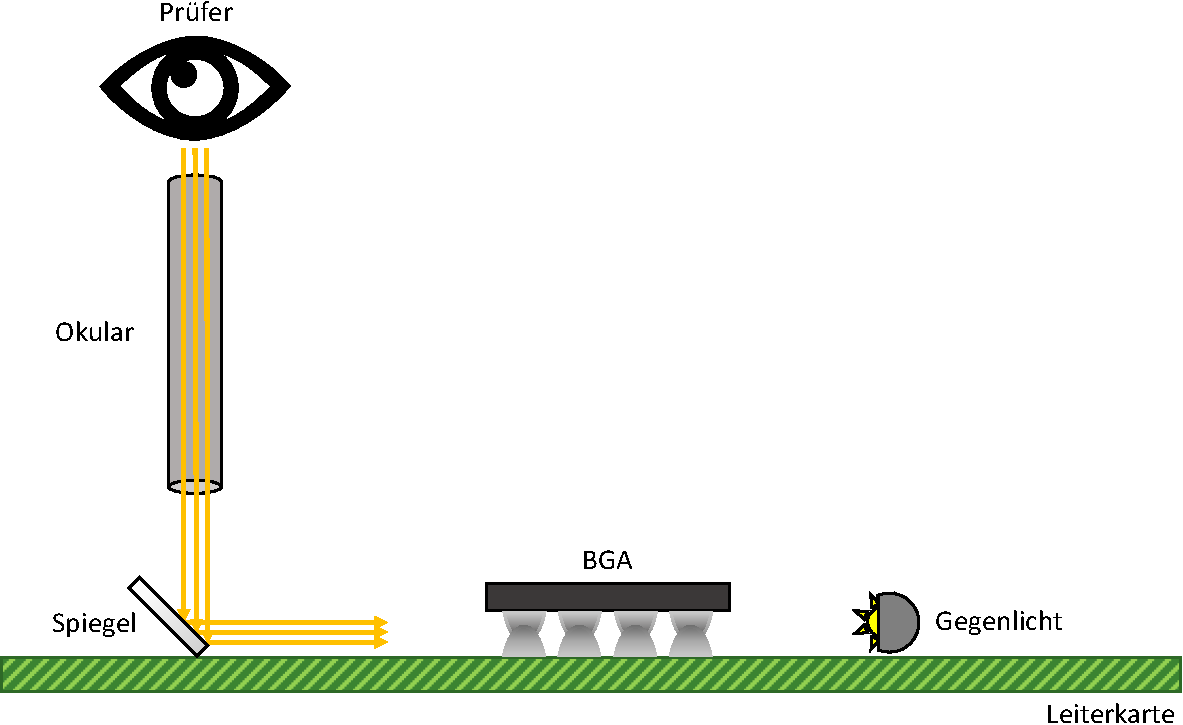
\includegraphics[width = \imgWidth, keepaspectratio = true]{Kapitel/Prüfverfahren in der Elektronikfertigung/Optische Prüfverfahren/Manuelle Optische Inspektion/Grafiken/BGA-InspektionFunktionsweise.pdf}
            \caption[Struktureller Aufbau eines \acs{bga}-Inspektionsgerätes]{Struktureller Aufbau eines \acs{bga}-Inspektionsgerätes. Mithilfe eines Spiegels können die Lötmenisken unterhalb des \acs{bga}-Chips betrachtet werden. In Anlehnung an: \cite{berger_test-_2012}}
            \label{Grafik: BGA-InspektionFunktionsweise}
        \end{figure}

        In der Regel weist dieser Inspektionskopf eine Tiefe von $1,5\,\si{\milli\metre}$ und eine Breite von $5\,\si{\milli\metre}$ bis $6\,\si{\milli\metre}$ auf.
        Die Tiefe ist entscheidend für die Lücke zwischen umliegenden Bauteilen und dem \ac{bga}.
        Die Breite ist ausschlaggebend, um die seitlich verfahrbare maximale Kantenlänge des \ac{bga}-Bausteins betrachten zu können.
        Meistens wird diese Länge durch umliegende Bauelemente limitiert (s. Abbildung \ref{Grafik: BGA-Inspektionsgeraet}). \cite{berger_test-_2012}

        Zur Ausleuchtung der ballförmigen Kontakte wird eine Kombination aus Front- und Gegenlicht verwendet.
        Das Frontlicht ist am Inspektionskopf angebracht und beleuchtet die am Rande und in erster Reihe liegenden Bälle.
        Aufgrund der direkten Beleuchtung ist die Betrachtung der Oberflächenstruktur, der Verbindungen und der Lötmenisken möglich.
        Zusätzlich können die \ac{bga}-Bälle auf Fehler, wie z.B. Mikrorisse, untersucht werden.  \cite{berger_test-_2012}

        Da sich die ballförmigen Kontake bei der Betrachtung gegenseitig optisch verdecken können, wird zusätzlich auch ein Gegenlicht eingesetzt.
        Diese Verdeckung ist in Abbildung \ref{Grafik: BGA-Inspektionsgeraet} in Form der Schatten erkenntlich. \cite{berger_test-_2012}

        \begin{figure}[htbp]
            \centering
            \includegraphics[width = 0.5\imgWidth, keepaspectratio = true]{Kapitel/Prüfverfahren in der Elektronikfertigung/Optische Prüfverfahren/Manuelle Optische Inspektion/Grafiken/BGA-Inspektionsgerät.pdf}
            \caption[Funktionsweise eines \acs{bga}-Inspektionsgerätes]{Funktionsweise eines \acs{bga}-Inspektionsgerätes. Die eingezeichneten Lichtstrahlen zeigen beobachtbare Punkte auf. In Anlehnung an: \cite{berger_test-_2012}}
            \label{Grafik: BGA-Inspektionsgeraet}
        \end{figure}

        Das Gegenlicht hilft bei der kontrastreicheren Darstellung der Form und Kanten innenliegender Lötbälle, da diese sonst aufgrund der Lichtabschottung durch dazwischenliegende Bälle nicht beleuchtet wären.
        Sowohl Front-, als auch das Gegenlicht sind seitlich synchron verfahrbar, sodass die einzelnen Durchgänge der Kontaktreihen nacheinander auf Lötbrücken oder Rückstände hin untersucht werden können. \cite{berger_test-_2012}

        Weiter ist der PC-unterstützte Bildvergleich als Hilfsmittel bei der \ac{moi} zu nennen.
        Zuerst wird das Golden Board und der Prüfling, z.B. mithilfe eines Scanners oder einer Kamera, in das Darstellungsprogramm auf dem Computer eingelesen.
        Dann wird der Prüfling und das Golden Board abwechselnd in einem bestimmten Intervall auf einem Monitor dargestellt.
        Durch den direkten Vergleich werden somit Unterschiede sichtbar dargestellt, die dann von der Prüfperson zu bewerten sind. \cite{berger_test-_2012}

    \minisec{Bewertung}
        Die \ac{moi} hat nach wie vor eine große Bedeutung in der Elektronikfertigung.
        Vorteilhaft ist, dass die \ac{moi} aus der Kategorie der optischen Prüfverfahren die größte Fehlerabdeckung besitzt. 
        Die Kosten, die initial für das Prüfen des Prüflings aufgewendet werden müssen, sind gering, da zum einen die Prüfmittel, wie ein Mikroskop - natürlich in Abhängigkeit der Leistungsfähigkeit - relativ kostengünstig erworben werden können und zum Anderen, da weitere Kosten, z.B. durch das Kaufen von Adaptern, das Anlernen von Personal, oder die Prüfprogrammerstellung wegfallen. \cite{berger_test-_2012}
        Zwar ist statt der Erstellung eines Prüfprogrammes die Erstellung eines Testplanes notwendig, damit keine möglichen Fehlerquellen bei der Kontrolle außer Acht gelassen werden, jedoch ist ein Prüfprogramm weitaus komplexer, da es richtige Eingabeparameter und genaue Instruktionen zur Prüfung braucht.
        Zudem ist der Mensch als lernfähiges Wesen dazu in der Lage, selbst Korrekturen am Prüfprozess anzufertigen, falls z.B. ein Prüfschritt fehlt und durch selbstständiges Handeln und Denken das Wissensrepertoire für weitere Prüflinge zu erweitern, falls ein neuer Fehler gefunden wurde - sozusagen als selbstoptimierender Prüfprozess \cite{berger_test-_2012}.

        Allerdings weist die selbstständige Auffassungsgabe auch einige Nachteile auf, die sich ausschlaggebend auf die Prüfqualität auswirken.
        Aufgrund unterschiedlicher Erfahrungen würde der selbe Prüfling zum Beispiel von zwei Prüfern unterschiedlich streng oder detailliert bewertet werden.
        Da der Prüfprozess aufgrund der manuellen Ausübung langwierig ist und viel Konzentration benötigt, treten bei der Prüfung oft Ermüdungserscheinungen in den Vordergrund, die zu einem großen Fehlerschlupf führen.
        Solche \glqq verschwindenden Fehler\grqq\@ und eine damit gleichzeitig einhergehende Qualitätsminderung entsprechen nicht dem Trend der stetig zunehmenden Zuverlässigkeitsanforderungen (s. Kapitel \ref{subsubsection: Motivation}).
        Die im Vergleich zur einer Maschine langsame Prüfgeschwindigkeit macht eine ausschließliche Nutzung der \ac{moi} nicht effizient, da sie, in der Produktionskette integriert, als das langsamste Glied zum Takttreiber wird.
        Deswegen ist die \ac{moi} nur für stichprobenartige Kontrollen, zur Erhebung einer Statistik dienend, oder zur Korrektur von Fehlern, die durch alternative Testverfahren detektiert worden sind, geeignet. \cite{berger_test-_2012}

        Zusätzlich sollen nun noch einmal die Kosten pro Prüfung beleuchtet werden.
        Da das Prüfverfahren eine ständige und genaue Aufmerksamkeit eines Prüfers voraussetzt, ist dieses sehr personalgebunden, sodass ein Mitarbeiter für einen wohlmöglich langen Zeitraum nicht für andere Aufgaben zur Verfügung steht.
        Gleichzeitig sind durch die aufgewandte Zeit auch die Personalkosten sehr hoch. \cite{berger_test-_2012}
        Diese hohen Personalkosten würden wiederum auf den Prüfling abgewälzt werden, sodass der Produktpreis steigen muss.

    \minisec{\acl{dft}}
        Damit die \ac{moi} bestmöglichst eingesetzt werden kann, müssen in der Entwicklungsphase der Leiterkarte bestimmte Punkte berücksichtigt werden.

        Die notwendige Bedingung ist, dass die auf Fehler zu untersuchenden Stellen auf der Leiterkarte frei sichtbar sein müssen.
        Um dies zu erreichen, sollten sich die Entwickler der Leiterkarte in die Prüfperson hineinversetzen, oder selbst eine Sichtkontrolle durchführen.
        Falls im Laufe des Fertigungsprozesses weitere Bauteile auf die Leiterkarte montiert werden, so bietet sich die prophylaktische Kontrolle der Leiterkarte im vorherigen Produktionsprozess an. \cite{berger_test-_2012}

            % Automatische Optische Inspektion
                \subsubsection{\acl{aoi}}
    Mit der fortschreitenden Leistungssteigerung von Computern und den dadurch verbesserten Möglichkeiten zur Prozessautomatisierung wurde auch die automatisierte Variante der Sichtkontrolle, die \ac{aoi}, zugänglich.
    Die Bauteile der Leiterkarten werden nunmals Schritt für Schritt, anhand eines Prüfprogrammes, mithilfe von Kameras inspiziert \cite{neumann_mut_2014}.
    
    Zusätzlich wurde der Ruf nach der \ac{aoi} größer, da der Einsatz der \ac{moi} in der Fertigung, aufgrund der niedrigen Geschwindigkeit und der fortschreitenden Miniaturisierung, an seine Grenzen gestoßen ist \cite{berger_test-_2012}.
    Der gestiegende Bedarf nach einer höheren Fertigungsqualität hat zudem die Erstellung von Prozessstatistiken und die damit verbundene, zur Rückkopplung notwendige, Dokumentationspflicht der Prüfergebnisse veranlasst, die in dem Umfang bei manuellen Prüftätigkeiten nicht tragbar ist.
    Da der vielseitige Einsatzzweck und die hohe Fehlerabdeckung der optischen Prüfverfahren dennoch weiterhin in der Fertigung eine große Rolle spielt, hat sich der Einsatz der \ac{aoi} im Laufe der Zeit als wesentlich zuverlässigere Prüfvariante herausgestellt \cite{berger_test-_2012}. 
    Im Gegensatz zur Sichtkontrolle werden \ac{aoi}-Systeme, aufgrund der höheren Geschwindigkeit, sowie einer konstanten Sorgfältigkeit bei der Prüfung, in den automatisierten Fertigungsprozess als sogenannte Inline-Testsysteme integriert und sind damit für verschiedenste Losmengen ausgelegt \cite{berger_test-_2012} \cite{stiny_fertigung_2010}.
    
    Dennoch ist die \ac{moi} in der Elektronikfertigung weiterhin ein unverzichtbares Mittel und geht teilweise Hand in Hand mit der automatischen optischen Inspektion einher.
    Neben dem Aufbau und der Funktionsweise solcher \ac{aoi}-Systeme, wird die enge Verknüpfung der \ac{aoi} und \ac{moi} in den folgenden Abschnitten näher beleuchtet.

    \minisec{Bestandteile eines \ac{aoi}-Systems}
        Ein System zur Durchführung einer automatischen optischen Inspektion lässt sich grob in zwei Funktionsbereiche, bestehend aus Hard- und Software gliedern.

        Die Hardwarebestandteile umfassen die optischen Elemente, wie die Kamera, Linsen und Beleuchtungen.

        Die Softwarekomponenten eines \ac{aoi}-Systems beinhalten die Mittel zur Steuerung des Prüfvorgangs anhand eines Prüfprogrammes, die Mittel zur Bewertung der Qualitätsmerkmale und die Mittel zur Verarbeitung und Speicherung der gewonnenen Daten.
        Da sich die Mittel zur Steuerung des Prüfvorgangs und die Mittel zur Verarbeitung und Speicherung der gewonnenen Daten zwischen Prüfverfahren ähneln, wird im Folgenden der Fokus auf die Softwarealgorithmen zur Bewertung der Qualitätsmerkmale gelegt.

    \minisec{Anforderungen an die Hardwarekomponenten}
        Die in ihrer Form und Farbe vielfältigen Bauteile, zum Teil auch die Anschlusspins auf einer Leiterkarte, erzeugen bei der Betrachtung in der optischen Inspektion ein kontrastreiches Bild.
        Dieses kontrastreiche Bild stellt die Bildaufnahme- und Bewertungsmechanismen vor große Herausforderungen.
        Aufgrund der zusätzlichen Abweichung der Helligkeitsmerkmale von Baugruppe zu Baugruppe besteht die Gefahr, dass Fehler nicht mehr zuverlässig erkannt werden, oder das eine ständige Anpassung des Prüfprogrammes notwendig ist, sodass die Automatisiertheit des Testsystems nicht mehr gegeben ist.
        Eine Prozessvariation führt somit schließlich auch zu einem unzuverlässigen Prüfverhalten, da mit ihr Veränderungen des optischen Verhaltens einhergehen. \cite{stiny_fertigung_2010}
        Dies schlägt sich in der Auswertung der Prüfmerkmale, durch die Auswertungsalgorithmen, nieder.
        Somit ist es im Vorfeld wichtig, die durch die Reflexionen erzeugten Unstimmigkeiten, durch eine hohe Bildaufnahmequalität, möglichst gering zu halten \cite{berger_test-_2012}.

        Daher bedarf es, zur Minimierung dieser Umstände, besonderen Optiken und Auswertungsalgorithmen, die im folgenden näher besprochen werden.

        Zunächst soll der Bildaufnahmemechanismus, als zentrales Element der \ac{aoi}, welcher die Bildinformationen in digitale Informationen umsetzt, besprochen werden.

        Zur Bildaufnahme in \ac{aoi}-Systemen kommen häufig Kameras, alternativ auch baugruppenbreite Scanner, zum Einsatz.
        Sie inspizieren das \ac{uut} meistens aus der Vogelperspektive, d.h. orthogonal zur Prüffläche, oder auch seitlich, sodass verdeckte Bereiche sichtbar werden.
        Die Kameras benötigen, um auch zwischen den kleinsten Bauteilen differenzieren zu können, eine hohe Pixelauflösung.
        Zur Bestimmung der benötigten Pixelauflösung wird das kleinste, zu Erkennung notwendige, Merkmal als Indikator genutzt. \cite{berger_test-_2012}

        Da man sich die Pixel des Kamerasenors als eine Art optischer Abtastpunkte vorstellen kann, muss zur Bestimmung der benötigten Pixelauflösung das Nyquist-Abttastheorem eingehalten werden.
        Zur Erkennung des kleinsten Merkmales mit einer bestimmten Breite muss dementsprechend die Pixelbreite weniger als die Hälfte der Merkmalbreite betragen.
        Im Umkehrschluss wird das Merkmal somit mit mindestens zwei Pixeln abgelichtet, sodass eine anschließende Darstellung möglich ist.
        Bei der Ablichtung von Lötmenisken empfiehlt es sich jedoch, die Pixelbreite fünf mal kleiner zu wählen. \cite{berger_test-_2012}

        Meistens werden zur Kompensation der hohen Pixelauflösung Vergrößerungsoptiken eingesetzt, da diese die effektiven Merkmalmaße vergrößern.
        Ein hochauflösendes Vollbild würde die Arbeitsgeschwindigkeit senken und den Speicherverbrauch drastisch erhöhen \cite{berger_test-_2012}.

        Durch die Vergrößerung und der damit einhergehenden Einschränkung des Sichtfeldes ist es für ein vollständiges Bild allerdings notwendig, das \ac{uut} in mehreren Schritten zu erfassen.
        Daher müssen die Kameras über ein X-Y-Achssystem verfahrbar sein.
        Dies hat Auswirkungen auf die für den prozesstaktgleichen Betrieb besonders zu berücksichtigende Prüfgeschwindigkeit des \ac{aoi}-Systems, da die Prüfmerkmale dann in mehr Schritten abgearbeitet werden müssen. \cite{berger_test-_2012}

        Weiter müssen die verwendeten Kameras, wie Eingangs erwähnt, die hohen Bildkontraste möglichst gut verarbeiten können.
        Zudem darf das Bild nicht durch Verzerrungen, Pixelfehler, oder Schwankungen auf Pixelebene (Grundrauschen, etc.), gestört werden, da die Auswertungsalgorithmen sonst Fehldeutungen treffen. 
        Daher ist für die optische Analyse auch ein stabiles Temperaturverhalten des Sensors notwendig. \cite{berger_test-_2012}

        Für die optische Erfassung des \ac{uut}, die Weiterverarbeitung der Daten und die Fehlerdiagnose ist auch der Bildfarbraum der Kameras entscheidend.
        So kann eine Aufnahme in \ac{sw} oder im \ac{rgb} Farbraum erfolgen. \cite{berger_test-_2012}

        Da die Bewertungsalgorithmen oft nur den Kontrast der Prüflingsmerkmale auswerten, wurden \acl{sw}-Kameras in der Vergangenheit sehr häufig eingesetzt \cite{berger_test-_2012}.
        Der häufige Einsatz der \ac{sw}-Kameras rührte aus einem geringeren Preis, im Vergleich zu Farbkameras mit gleicher Auflösung.
        Eine farbliche Unterscheidung der Komponenten wurde durch eine farbige Beleuchtung erreicht \cite{berger_test-_2012}.
        Auch waren die Übertragungsbandbreite, sowie die Systemleistung zur Verarbeitung und Auswertung, wichtige Faktoren zum Entscheid für eine \ac{sw}-Kamera \cite{berger_test-_2012}.
        Mittlerweile wurden die \ac{sw}-Kameras vom Markt fast vollständig verdrängt \cite{berger_test-_2012} und eine farbige Ablichtung ist trotzdem, durch bestimmte Verfahren, zu einem niedrigen Preis möglich.
        Bei der \ac{aoi} ist jedoch entscheidend, mit welchem Verfahren die Farbinformationen für die bildliche Darstellung entstehen, da es bei den hohen Auflösungen aufgrund unerwünschter Effekte zu Fehlinterpretationen kommen kann \cite{berger_test-_2012}.

        Ein verbreiteter kostengünstiger Farbkameratypus ist die 1-Chip-Kamera.
        Wie der Name schon vermuten lässt, wird zur Bildaufnahme nur ein Sensor benötigt.
        Die jeweiligen \ac{rgb}-Farbkanäle werden durch ein spezielles Farbfiltergitter auf den Pixeln, dem Bayer-Filter-Array, aus dem von dem \ac{uut} reflektierten Licht herausgefiltert.
        Um die höhere Lichtempfindlichkeit des menschlichen Auges gegenüber grünem Licht in die Bildaufnahme einfließen zu lassen, liegen die Pixel in einem 1R:2G:1B Verhältnis vor.
        Das Verfahren, um aus diesen Subpixeln den eigentlichen Farbwert zu berechnen, wird als Bayer-Demosaicing bezeichnet.
        Beim Bayer-Demosaicing werden die benachbarten Pixel zur Berechnung des Zwischenwertes herangezogen.
        Unter Umständen führt dies allerdings zu einer drastischen Reduzierung der Ortsauflösung (nur noch $\frac{1}{4}$ der ursprünglichen Auflösung), da dann nur eines dieser Subpixel das Licht eines Merkmales empfängt.
        Da die farbliche Abdeckung durch das veränderte Subpixelverhältnis nun verändert ist, zeigt sich ein Artefakteproblem, das der Auswertungsalgorithmus nur unzuverlässig deuten kann. \cite{berger_test-_2012}

        Als Alternative werden in den \ac{aoi}-Systemen 3-Chip-Kameras verwendet.
        Hierbei werden, zur Elimination der Farbartefakte bei einer hohen Ortsauflösung, drei separate \ac{sw}-Bildsensoren genutzt, die das Bild für einen Farbkanal des \ac{rgb}-Farbraums ablichten.
        Dabei sorgt ein Prisma für die korrekte Aufteilung des Lichtes in die Grundfarben Rot, Grün und Blau und leitet diese Farben an den jeweiligen Bildsensor.
        Durch diese Aufteilung behält man die hohe Ortsauflösung bei, da die Ablichtung im jeweiligen \ac{rgb}-Farbkanal für den jeweiligen Sensor in \acl{sw} erfolgt. 
        Durch die dreifache Ablichtung pro Bildpunkt werden somit auch die Farbartefakte vermieden. \cite{berger_test-_2012}
        Da für den jeweiligen Farbkanal nun die Intensität der Pixel als Wert vorliegt, erfolgt die Rekonstruktion der Farbinformationen durch das Zusammenfügen der jeweiligen Farbwerte zu einem 3-Tupel (\ac{rgb}-Farbwerte) pro Pixel.
        3-Chip-Kameras sind aufgrund der dreifachen Hardwareausführung teuerer als 1-Chip Lösungen und benötigen mehr Einbauplatz, da zusätzlich zu dem Prisma noch Korrekturoptiken zur Optimierung des Lichtdurchgangs verwendet werden müssen \cite{berger_test-_2012}.

        Kostengünstiger und platzsparender, unter Beibehaltung der hohen Ortsauflösung, ist die sequentielle Ablichtung des Prüfobjektes durch eine einzelne \acl{sw}-1-Chip-Kamera.
        Hierbei werden die Informationen über die Farbkanäle nicht anhand einer direkten Aufspaltung des Lichtes erreicht, sondern man macht sich die Absorption und Reflexion des sequentiell ausgestrahlten, unterschiedlich farbigen Lichtes zu nutzen.
        Hieraus erhält man, ähnlich wie bei den 3-Chip-Kameras, durch eine Wertezusammensetzung, den jeweiligen Pixelfarbwert. \cite{berger_test-_2012}
        Das Prüfobjekt darf sich allerdings während der Ablichtung und Zusammensetzung nicht bewegen, da das Bild sonst verschmiert.
        
        Da die Bildqualität nicht nur wesentlich durch die Kameraeigenschaften beeinflusst wird, sondern die Optik im Vorfeld das eingestrahlte Licht der Leiterkarte verändert, bevor es zur Detektion auf die Bildpunkte des Sensors trifft, ist die Optik im Vorfeld für eine hohe Bildqualität hauptzuständig.
        Aufgrund der nicht-idealen Eigenschaften der Optik kommt es bei der Übersetzung des Objektpunktes zu einem Bildpunkt zu Fehlern, die sich als \glqq Fleck\grqq\@ bemerkbar machen. \cite{berger_test-_2012}

        Die Auflösung, die optische Verzerrung, sowie die Güte der Optik zählen zu den ausschlaggebensten Eigenschaften, die die Bildqualität bestimmen und zur Fleckenminimierung zu optimieren sind \cite{berger_test-_2012}. 
        Diese sollen nun im Folgenden besprochen werden: 

        \begin{enumerate}
            \item \textbf{Auflösung:} Für die letzendlich zu erreichende Auflösung ist die Betrachtung der Parameter einer Optik wichtig, die für die Abbildungsgröße des Merkmales verantwortlich sind \cite{berger_test-_2012}.
            \item \textbf{Verzerrung:} Die Verzerrung setzt sich aus der perspektivischen Ansicht und dem möglichen erreichbaren Schärfentiefenbereich zusammen. Da bei der Betrachtung des \ac{uut} das Sichtfeld der Optik vollständig bedeckt ist und der Auswertungsalgorithmus unter gleichbleibenden Inspektionsbedingungen die zuverlässigsten Ergebnisse liefert, muss das \ac{uut}, unabhängig der Lage und Position, immer gleich abgebildet werden. Daher darf die Betrachtungsperspektive nur geringfügige Auswirkungen auf das Prüflingsbild haben. Der Schärfentiefebereich
            \item \textbf{Güte:}
        \end{enumerate} 

        Verzeichnung (Perspektivität, Schärfentiefebereich); Güte (optische Fehler, Beugungsfehler)
        \cite{berger_test-_2012}

        \minisec{Anforderungen an die Softwarekomponenten}
%%%%%%%%%%%%%%%%%%%%%%%%%%%%%%%%%%%%%%%%%%%%%%%%%%%%%%%%%%%%%%%%%%%%%%%%%%%%

    \newpage

%%%%%%%%%%%%%%%%%%%%%%%%%%% Literaturverzeichnis %%%%%%%%%%%%%%%%%%%%%%%%%%%
    \printbibliography
%%%%%%%%%%%%%%%%%%%%%%%%%%%%%%%%%%%%%%%%%%%%%%%%%%%%%%%%%%%%%%%%%%%%%%%%%%%%

    \newpage

%%%%%%%%%%%%%%%%%%%%%%% Eidesstattliche Versicherung %%%%%%%%%%%%%%%%%%%%%%%
    Eidesstattliche Versicherung
%%%%%%%%%%%%%%%%%%%%%%%%%%%%%%%%%%%%%%%%%%%%%%%%%%%%%%%%%%%%%%%%%%%%%%%%%%%%

%----------------------------- Prototypisches -----------------------------%
    % Grobe Gliederung
        % \setcounter{section}{0}

\section{Einleitung}
    Dieses Praxisprojekt entsteht in der Zusammenarbeit mit der Trützschler Group SE in Mönchengladbach Odenkirchen\dots

    \subsection{Die Trützschler Group}

        \annot{Unternehmen vorstellen}

        \annot{Was macht Trützschler?}

        \annot{Was ist das besondere bei Trützschler?}

    \subsection{Problemstellung}

        \annot{TSAS ist alt}

            \annot{Keine Ersatzteile mehr für TSAS}
            
            \noindent
            \annot{Software}

                \annot{Keine Updates mehr}

                \annot{Es ist schwierig neue Leiterkarten dort einzubinden}

                \annot{Neues System nutzt bestehende CAD-Dateien}

            \noindent
            \annot{Adapterbau ist teuer und aufwendig}

                \annot{Beispiel anbringen für den Preis und den Aufwand (Euro und Stunden)}

                \annot{Debugging der Adapter ist auch aufwendig}
                
                \annot{Daher sollen alte Adapter auf dem neuen System funktionieren}

    \subsection{Ziele des Praxisprojektes}

        \annot{Mir einen Einblick in den Ablauf der industriellen Produktion von Leiterkarten geben}

        \noindent
        \annot{Über verschiedene Testmöglichkeiten informieren}

        \noindent
        \annot{R\&S und SPEA dokumentieren}

        \noindent
        \annot{Maschinen kennenlernen}

            \annot{Gemeinsamkeiten und Unterschiede der Tester erfahren}

            \annot{Mögliche Migrationsstrategien stellen sich dabei heraus}

    \subsection{Aufbau des Praxisprojektes}

\section{Testverfahren in der Industrie}

    \subsection{Herstellungsschritte der Leiterkarten}

        \annot{Unbestückte Leiterkarte/PCB heißt dann PCBA (Printed Circuit Board Assembly)}

        \noindent
        \annot{Von der Planung bis zur fertigen Karte}

            \annot{\notsure{Vielleicht als Flussdiagramm?}}

            \annot{Bestückungsreihenfolge}

                \indent \indent \annot{Hinsichtlich der Bauelemente}

            \annot{Verschiedene Testverfahren, die durchlaufen werden}

                \indent \indent \annot{Von dem ICT mit Kurzschlusstest (sehr am Anfang) bis hin zur Wärmekammer}

                    \indent \indent \indent \annot{\notsure{Vielleicht als Flussdiagramm?}}

        \noindent
        \annot{\notsure{Wie designed man for Test?}}

            \annot{Regeln aufführen}

            \annot{Unter dem Aspekt, dass einige Leiterkarten nicht ICT fähig sind}

                \indent \indent \annot{Hohe Bauteile}

                \indent \indent \annot{Bottom Bestücktheit}

                \indent \indent \annot{Wie wird mit solchen Boards verfahren? \notsure{Flying Probe?}}

    \subsection{Notwendigkeit der Testverfahren}

        \annot{Fehler die auftreten können (Fehlerarten/Fehlertypen) und dann sagen, dass das Testen sinnvoll ist}

            \annot{Z.B. kann ein Widerstand falsch sein/Bauteilwert falsch sein}

                \indent \indent \annot{Würde man erstmal so nicht drauf kommen}

            \annot{Bei BGA ist ein Pin nicht richtig verlötet}

                \indent \indent \annot{Würde man erstmal so nicht drauf kommen}

        \noindent
        \annot{Statistik ansprechen, wieviele Leiterkarten gebaut werden}

            \annot{Sagen wieviele davon durchfallen}

            \noindent
            \annot{Grund ist die Qualitätssicherung, Kostenminimierung und Sicherheit für die Inbetriebnahme}

                \indent \annot{Durch das Testen können außerdem Verbesserungen an dem Produkt vorgenommen werden}

                \indent \annot{Das ganze mit Minisections gliedern}

    \subsection{Testverfahren}

        \subsubsection{Standard In Circuit Testing \dbg{<- Acronym}}

            \annot{Manufacturing Defect Analysis (MDA)}

            \noindent
            \annot{Design-for-Testability}
                \notsure{Nochmals anschneiden und spezifische Werte füllen?}

            \noindent
            \annot{Adapter}

                \annot{Single Bay oder Dual Bay}

                \annot{Nadelarten}

            \noindent
            \annot{Single Core und Multi Core Systeme}

        \subsubsection{Flying Probe Testing}

        \subsubsection{BIST}

        \subsubsection{Optische Testverfahren}

            \annot{Man kann die Polarität von Elkos nicht messtechnisch bestimmen, daher ist das hier sinnvoll!}

            \noindent
            \annot{Manuelle Optische Inspektion}

            \noindent
            \annot{Automatische Optische Inspektion}

        \subsubsection{Röntgeninspektion}

        \subsubsection{\notsure{Funktionstest}}

        \subsubsection{\notsure{Zusätzliche Features wie ISP}}

        \subsubsection{weitere Recherche nötig\dots \annot{Weitere und gucken ob es auch VERFAHREN sind!}}

    \subsection{Teststrategien}

        \subsubsection{Kapazitäten \annot{Wie kann man die Kapazität/andere Bauteile messen}}

            \annot{Dieser Teil hier soll unabhängig des Testverfahrens sein}

                \annot{\notsure{Also ist der Boundary Scan zu den oberen Punkten (ICT, FPT, usw.) zugehörig?}}

        \subsubsection{Analoger Test}

            \annot{\notsure{Vectorless?}}
            
            \noindent
            \annot{\notsure{Hier Open Pin Test als Alternative für den Digitaltest anführen?}}

                \indent \annot{\notsure{Digitaltest benötigt ja hohe Schaltfrequenzen und perfektes Timing}}

                \indent \annot{\notsure{Werden feste Testmuster (bekannte Ein- und Ausgabe) benötigt?}}

        \subsubsection{Digitaler Test}

            \annot{\notsure{Vector Test?}}

            \noindent
            \annot{\notsure{Bei Geräte die keinen Boundary Scan unterstützen?}}

        \subsubsection{Mixed Signal Test}

        \subsubsection{Boundary Scan (JTAG)}

            \annot{Boundary Scan Descriptive Language}

        \subsubsection{Junction Scan/Open Pin Test}

        \subsubsection{Funktionstest}

    \subsection{Maßnahmen zur Messfehlerreduzierung}

        \subsubsection{Guarding}

            \annot{Laut T.W. gibt es hierfür mehrere Möglichkeiten}

        \subsubsection{Mehrdrahtmessung}

        \subsubsection{weitere Recherche nötig\dots}

\section{Praxisbeispiele}

    \subsection{Rohde \& Schwarz TSAS}
        \subsubsection{Grundlegendes}

        \subsubsection{Aufbau/Funktionsweise/Schnittstellen}

        \subsubsection{Module/Technische Spezifikationen}

        \subsubsection{Besonderheiten}

        \subsubsection{Probleme}

    \subsection{SPEA 3030 Compact}
        \subsubsection{Grundlegendes}
        
        \subsubsection{Aufbau/Funktionsweise/Schnittstellen}

            \annot{Augat Pylon Interface}

        \subsubsection{Module/Technische Spezifikationen}

        \subsubsection{Besonderheiten \annot{Stray Capacitance Ausgleich z.B.}}

        \subsubsection{Probleme}

    \subsection{Kompatibles}

        \subsubsection{Vorschläge, wie die Migration erfolgen könnte (in der BA prüfen und sich entscheiden?)}

    \subsection{Unterschiede/Inkompatibilitäten}

        \subsubsection{Wie könnte man damit verfahren (in der BA ansprechen und einen Weg raussuchen?)}

\section{Zusammenfassung}

\section{Ausblick}

    \noindent
    \annot{Ausblick über allgemeine Testverfahren}

    \noindent
    \annot{\notsure{Ausblick über die Verfahrenswege der Migration}}

\section{Fazit}

    % Weitere Gliederung
        % \setcounter{section}{0}

\section*{Einleitung}

    \subsection*{Vorwort}

    \subsection*{Problemstellung}

    \subsection*{Ziele des Praxisprojektes}

        \annotdone{Mir einen Einblick in den Ablauf der industriellen Produktion von Leiterkarten geben}

        \noindent
        \annotdone{Über verschiedene Testmöglichkeiten informieren}

        \noindent
        \annotdone{R\&S und SPEA dokumentieren}

        \noindent
        \annotdone{Maschinen kennenlernen}

            \annotdone{Gemeinsamkeiten und Unterschiede der Tester erfahren}

            \annotdone{Mögliche Migrationsstrategien stellen sich dabei heraus}

    \subsection*{Aufbau des Praxisprojektes}

\section*{Die Trützschler Group}

    \subsection*{Allgemeines}

        \annotdone{Jetzigen Text mit etwas geschichtlichem Hintergrund füllen}

    \subsection*{Geschäftszweige}

        \annot{Mit Bildern füllen}

    \subsection*{Besonderheiten}

        \annotdone{Fast alles wird selber hergestellt}

        \annotdone{Hochqualitative Leiterkartenproduktion in DEUTSCHLAND}

\section{Prüfverfahren in der Elektronikfertigung}

    \annot{Kriterien für die Testverfahren siehe blunk-electronic oder Kärger}

    \subsection*{Notwendigkeit der Prüfverfahren}

        \annot{Statistik ansprechen, wieviele Leiterkarten gebaut werden}

            \annot{Sagen wieviele davon durchfallen}

        \noindent
        \annotdone{Grund ist die Qualitätssicherung, Kostenminimierung und Sicherheit für die Inbetriebnahme}

            \indent \annotdone{Durch das Testen können außerdem Verbesserungen an dem Produkt vorgenommen werden}

            \indent \annotdone{Zum Punkt Kostenminimierung: Rule Of Ten oder Kärger die $10^{s}$ Formel.}

            \indent \annotdone{Das ganze mit Minisections gliedern}

    \subsection*{Fehler}

        \annotdone{Fehler die auftreten können (Fehlerarten/Fehlertypen) und dann sagen, dass das Testen sinnvoll ist}

            \annotdone{Z.B. kann ein Widerstand falsch sein/Bauteilwert falsch sein}

                \indent \indent \annotdone{Würde man erstmal so nicht drauf kommen}

        \annotdone{Bei BGA ist ein Pin nicht richtig verlötet}

            \indent \indent \annotdone{Würde man erstmal so nicht drauf kommen}

    \subsection{Phasen des Herstellungsprozesses}

        \annot{\notsure{Stiny Buch hier nützlich?}}

        \annot{\notsure{Sicherheitskritische Tests, z.B. Schutz vor Berührungen von 230V garantieren; Hierzu Normen o.ä. finden}}

        \noindent
        \annot{Wann muss/sollte getestet werden}

            \annot{Hierzu die Präsentation von blunk-electronic!}
        
        \noindent
        \annot{Unbestückte Leiterkarte/PCB heißt dann PCBA (Printed Circuit Board Assembly)}

        \noindent
        \annot{Von der Planung bis zur fertigen Karte}

            \annot{\notsure{Vielleicht als Flussdiagramm?}}

            \annot{Bestückungsreihenfolge}

                \indent \indent \annot{Hinsichtlich der Bauelemente}

            \annot{Verschiedene Testverfahren, die durchlaufen werden}

                \indent \indent \annot{Von dem ICT mit Kurzschlusstest (sehr am Anfang) bis hin zur Wärmekammer}

                    \indent \indent \indent \annot{\notsure{Vielleicht als Flussdiagramm?}}

        \subsubsection{Entwicklungsphase}

            \annot{Design For Test anführen}

            \annot{Warum ist Design For Test so wichtig?}

            \noindent
            \annot{Wie designed man for Test?}

            \noindent
            \annot{Grundlegende Regeln aufführen}

                \annot{Weitere und speziellere Regeln bei dem jeweiligen Verfahren nennen}

            \noindent
            \annot{Unter dem Aspekt, dass einige Leiterkarten nicht ICT fähig sind}

                \indent \indent \annot{Hohe Bauteile}

                \indent \indent \annot{Bottom Bestücktheit}

                \indent \indent \annot{Wie wird mit solchen Boards verfahren? \notsure{Flying Probe?}}

        \subsubsection{Produktionsphase}

        \subsubsection{Verifikationsphase}

            \annot{Testen der Leiterkarten}

    \subsection{Optische Prüfverfahren}

        \annot{Man kann die Polarität von Elkos nicht messtechnisch bestimmen, daher ist das hier sinnvoll!}

        \subsubsection{Manuelle Optische Inspektion}

            \annot{Design For Test}

        \subsubsection{Automatische Optische Inspektion}

            \annot{Design For Test}

        \subsubsection{Röntgeninspektion}

            \annot{Design For Test}

    \subsection{Elektrische Prüfverfahren}

        \subsubsection{In Circuit Testing}

            \annot{Manufacturing Defect Analysis (MDA)}

            \annot{Prüfparameter der Bauelemente \refneeded{-> (Kärger/K4SK1)}}

            \noindent
            \annot{Design-for-Testability}
                \notsure{Nochmals anschneiden und spezifische Werte füllen?}

            \noindent
            \annot{Adapter}

                \annot{Single Bay oder Dual Bay}

                \annot{Nadelarten}

            \noindent
            \annot{Single Core und Multi Core Systeme}

            \annot{Design For Test}

        \subsubsection{Flying Probe Testing}

            \annot{Design For Test}

        \subsubsection{Funktionstest}

            \annot{Eigentlich ist hierfür doch ein OBP (On Board Programming) mit \notsure{ISP?} nötig?}

            \noindent
            \annot{Design For Test}

        \subsubsection{Build in self Test}

            \annot{Eigentlich ist hierfür doch ein OBP (On Board Programming) mit \notsure{ISP?} nötig?}

            \noindent
            \annot{Design For Test}

    \subsection{Messstrategien}

        \subsubsection{Analoger Test}

            \annot{Wie kann man die Kapazität/andere Bauteile messen}

            \noindent
            \annot{\notsure{Vectorless?}}

            \noindent
            \annot{\notsure{Hier Open Pin Test als Alternative für den Digitaltest anführen?}}

                \indent \annot{\notsure{Digitaltest benötigt ja hohe Schaltfrequenzen und perfektes Timing}}

                \indent \annot{\notsure{Werden feste Testmuster (bekannte Ein- und Ausgabe) benötigt?}}
        
            \noindent
            \annot{Maßnahmen zur Messfehlerreduzierung}

                \annot{Guarding}

                    \annot{Laut T.W. gibt es hierfür mehrere Möglichkeiten}

                \annot{Vierdrahtmessung/Kelvinmessung}

                \annot{\notsure{Stromrichtige Messung}}

                \annot{\notsure{Spannungsrichtige Messung}}

        \subsubsection{Digitaler Test}

            \annot{\notsure{Vector Test?}}

            \noindent
            \annot{\notsure{Bei Geräte die keinen Boundary Scan unterstützen?}}

        \subsubsection{Mixed Signal Testing}

        \subsubsection{Junction Scan/Open Pin Scan}

        \subsubsection{Boundary Scan (JTAG)}

            \annot{Verschiedene IEEE Standards nennen von .1 bis .4 analog boundary scan}
            
            \noindent
            \annot{Boundary Scan Descriptive Language}

\section{Praxisbeispiel: Rohde \& Schwarz TSAS}

    \subsection{Grundlegende Informationen}

    \subsection{Aufbau}

        \annot{Augat Pylon Interface}

    \subsection{Funktionsweise}

    \subsection{Technische Spezifikationen}

        \subsubsection{Module}

        \subsubsection{Schnittstellen}

    \subsection{Besondere Merkmale}

    \subsection{Probleme}

\section{Praxisbeispiel: SPEA 3030 Compact}

    \subsection{Grundlegende Informationen}

    \subsection{Aufbau}

        \annot{Augat Pylon Interface}

    \subsection{Funktionsweise}

    \subsection{Technische Spezifikationen}

        \subsubsection{Module}

        \subsubsection{Schnittstellen}

    \subsection{Besondere Merkmale}

        \annot{Stray Capacitance Ausgleich z.B.}

    \subsection{Probleme}

\section{Kompatibilität und mögliche Verfahrenswege}

    \annot{Vorschläge, wie die Migration erfolgen könnte (in der BA prüfen und sich entscheiden?)}

    \noindent
    \annot{Inkompatibles}

        \annot{Wie könnte man damit verfahren (in der BA ansprechen und einen Weg raussuchen?)}

\section{Zusammenfassung}

\section{Ausblick}

    \noindent
    \annot{Ausblick über allgemeine Testverfahren}

    \noindent
    \annot{\notsure{Ausblick über die Verfahrenswege der Migration}}

\section{Fazit}

    % To-Do-Liste
        \newpage
\section*{\dbg{To-Do-Liste}}
    \begin{itemize}
        \item Acros hinzufügen und prüfen!
        \item Jahreszahlen fehlen bei Bücherquellen (o.D.)
        \item Boxen um die hyperlinks entfernen, weil die sonst im Druck oder auf anderen Geräten auftauchen!
        \item Seitenzahl links und rechts mit section und subsection links und rechts abwechselnd gestalten!
    \end{itemize}

    % Testseite
        % \newpage
Hier sind alle Debugging-Befehle benutzt worden:

\annot{Anmerkung} (Textlich/Inhaltliche Anmerkung)

\citneeded{IGrout06} (Bei fehlendem Zitat)

\refneeded{->2.1.4} (Bei fehlender Referenz)

\dbg{Debugnachricht} (Dokumententechnische Anmerkung)

\dbg{Achtung! Ab hier wird der Section- und Page-Zähler resettet!}

\setcounter{section}{0}
\setcounter{page}{1}

\newpage

\begin{center}
    \begin{minipage}{0.75\textwidth}
        \section*{Abstract}
            Komplexe Zahlen sind aus der heutigen Welt kaum wegzudenken.
            Sie sind zur Bewältigung trivialer Dinge, wie die komplexe Wechselstromrechnung, bis hin zu technisch herausfordernden Aufgaben, wie der Signalverarbeitung nötig.
    \end{minipage}
\end{center}

\section{Einleitung}
Dieses Praxisprojekt entsteht in der Kooperation mit der Trützschler Group SE in Mönchengladbach Odenkirchen.
Die Trützschler Group ist das beste Unternehmen im Bereich der Textilmaschinenherstellung.

\begin{center}
    \begin{minipage}[t]{0.3\textwidth}
        Das ist ein \textbf{minipage} Test, um zu schauen, was dies für Auswirkungen hat.
    \end{minipage} 
    \hspace{0.3\textwidth}
    \begin{minipage}[t]{0.3\textwidth}
        Das ist die zweite \textbf{minipage} auf dieser Seite.
    \end{minipage}
\end{center}

Verantwortliche Wissenschaftler haben herausgefunden, sind danach direkt aber wieder in die ETH\footnote{Die ETH-Zürich ist eine Hochschule in der Schweiz, die sich durch laute Porsche Cayenne Fahrer vom Rest der Welt abhebt.}-Zürich hineingewandert, da es geregnet\footnotemark[1] hat.

\begin{center}
    \begin{minipage}[t]{\textwidth}
        \begin{center}
            \fbox{$Z_{in} = (1 + \imath \frac{A_{ac}}{\sqrt{1 + \imath}}) \Omega$}   
        \end{center}
    \end{minipage} 
\end{center}

\section{Problemstellung}
Problem ist, dass viele Leute einfach abgehoben\footnotemark\@ sind.
\footnotetext{Ich musste die Befehle trennen, da auf dieser Seite sowieso alles schon verrückt ist.}
\cite{berger_test-_2012}\cite{grout_integrated_2006}\cite{karger_pruftechnik_1985}\cite{stiny_fertigung_2010}



    
    % Layout
        % \layout{} % Zeigt eine Übersicht der im Dokument vorhandenen Längen samt Zahlenwerte an.
%----------------------------- Prototypisches -----------------------------%

\end{document}